\chapter{Metodolog'ia}

\section{Sistema de control}

\subsection{Funci'on de Transferencia}

\abovedisplayskip=0pt
\belowdisplayskip=0pt

El controlador est'a basado en un sistema de equilibrio en bajo o mejor llamado \textit{Down-position} o \textit{crank-down}; y cuya funci'on de transferencia obtenida en la tesis previa de \citet{montalvo}:
\setlength{\parskip}{0pt}
\begin{equation}\label{eq:1} 
\,\ddot{x}=\frac{F-ml(\ddot{\theta}\cos\theta+\dot{\theta}^{2}\sin{\theta})-f_{c}\dot{x}}{(M+m)}\\
\end{equation}
\myequations{Funci'on de transferencia aceleraci'on lineal}
\begin{equation}\label{eq:2}
\,\ddot{\theta}=\frac{mgl\sin{\theta}-ml\ddot{x}\cos{\theta}-f_{p}\dot{\theta}}{(I_{p}+ml^{2})}
\end{equation}
\myequations{Funci'on de transferencia aceleraci'on angular}
\setlength{\parskip}{0.4cm}
Cuyos par'ametros estan representados en el cuadro \ref{parametros} y son:
\begin{table}[ht]
\centering
\begin{tabular}{ll}
$x_{p}$ &  X-coordinate for center of gravity of pendulum.\\
$y_{p}$  & Y-coordinate for center of gravity of pendulum.\\
$x_{c}$  & X-coordinate for center of gravity of cart.\\
$y_{c}$  & Y-coordinate for center of gravity of cart.\\
$y_{pp}$  & Y-coordinate for pivot point.\\
$l$  & Distance from pendulum center of gravity to pivot point.\\
$\theta$  & Pendulum angle from positive Y-direction.\\
$m$  & Mass of pendulum (load and rod).\\
$M$  & Cart mass.\\
$F$  & Force applied to cart.\\
$V$  & Vertical reaction force from pendulum.\\
$H$  & Horizontal reaction force from pendulum.\\
$I_{p}$  & Moment of inertia for pendulum with respect to pivot point.\\
$f_{p}$  & Viscous friction for pendulum at pivot point.\\
$f_{c}$  & Dynamic friction for cart.\\
 
\end{tabular}
\caption{Par'ametros de la funci'on de transferencia}
\label{parametros}
\end{table}


\section{Punto de equilibrio del sistema}
La ecuaci'on \ref{eq:1} muestra la representaci'on del sistema de una forma no-lineal. 
Equilibrio est'a definido como un punto (o una curva) en donde todos los estados permanecen sin cambio, sus derivadas son ceros (0). Despu'es de que \ref{eq:1} haya sido reemplazada en \ref{eq:2} y viceversa aparece un nuevo sistema de ecuaciones: \\

\setlength{\parskip}{0pt}

\begin{equation}\label{eq:3}
\,\beta\ddot{x}=(I_{p}+ml^{2})(F+ml\dot{\theta}^{2}\sin{\theta}-f_{c}\dot{x})-ml\cos{\theta}(mgl\sin{\theta}-f_{c}\dot{\theta})
\end{equation}
\myequations{Ecuaci'on de equilibrio 1}

\begin{equation}\label{eq:4}
\,\beta\ddot{\theta}=(M+m)(mgl\sin{\theta}-f_{p}\dot{\theta})-ml\cos{\theta}(F+ml\dot{\theta}^{2}\sin{\theta}-f_{c}\dot{x}) 
\end{equation}
\myequations{Ecuaci'on de equilibrio 2}
\begin{equation}\label{eq:5}
\,\beta=(M+m)(I_{p}+ml^{2})-(ml\cos{\theta})^{2} 
\end{equation}
\myequations{Ecuaci'on de equilibrio 3}
\setlength{\parskip}{0.4cm}
Las condiciones de $\dot{x}=0$,$\dot{\theta}=0$ y $F=0$ entonces las ecuaciones \ref{eq:3} y \ref{eq:4} resultan:\\
\setlength{\parskip}{0pt}
\begin{equation}\label{eq:6}
\,\beta\ddot{x}=-ml\cos{\theta}(mgl\sin{\theta}-f_{c}\dot{\theta})=0
\end{equation}
\myequations{Ecuaci'on de equilibrio 1 con condiciones iniciales 0}
\begin{equation}\label{eq:7}
\,\beta\ddot{\theta}=(M+m)(mgl\sin{\theta})=0
\end{equation}
\myequations{Ecuaci'on de equilibrio 2 con condiciones iniciales 0}
\setlength{\parskip}{0.4cm}
Ya que $\beta\neq0$ los 'unicos puntos que satisfacen estas ecuaciones son $\theta=0$ y $\theta=\pi$.
Esto tiene sentido ya que el p'endulo puede permanecer directamente abajo; as'i como hacia arriba si nada lo perturba.

\subsection{Linealizaci'on en posici'on bajo}
Si el 'area enfocada para el controlador en bajo es ($\theta=\pi$, $\dot{\theta}_{0}=0$), entonces tiene sentido linealizar para estos puntos, definiendo $\theta$ como una desviaci'on de $\theta_{\pi}$.La linealizaci'on usando las series de Taylor se muestra a continuaci'on.
\setlength{\parskip}{0pt}
\begin{equation}\label{eq:8}
\,\sin{\theta} \approx \sin{\theta}_{0}+ \left. \frac{\mathrm{d} \sin{\theta}_{0}}{\mathrm{d} x}\right|_{\theta_{0}=\pi} *\theta + \varepsilon \approx 0-1*\theta=-\theta
\end{equation}
\myequations{Taylor $\sin{\theta}$}
\setlength{\parskip}{0.4cm}
\setlength{\parskip}{0pt}
\begin{equation}\label{eq:9}
\cos{\theta} \approx \cos{\theta}_{0}+ \left. \frac{\mathrm{d} \cos{\theta}_{0}}{\mathrm{d} x}\right|_{\theta_{0}=\pi} *\theta + \varepsilon \approx -1-0*\theta=-1
\end{equation}
\myequations{Taylor $\cos{\theta}$}
\setlength{\parskip}{0.4cm}

Para $(\theta_{0}=\pi,\dot{\theta_{0}}=0)$ las versiones de ecuaciones linealizadas de las ecuaciones \ref{eq:8} y \ref{eq:9} son:
\setlength{\parskip}{0pt}
\begin{equation}\label{eq:10} 
\,\ddot{x}=\frac{F+ml\ddot{\theta}-f_{c}\dot{x}}{(M+m)}\\
\end{equation}
\myequations{Funci'on de transferencia lineal de $\ddot{x}$}
\begin{equation}\label{eq:11}
\,\ddot{\theta}=\frac{-mgl\theta-ml\ddot{x}-f_{p}\dot{\theta}}{I_{p}+ml^{2}}
\end{equation}
\myequations{Funci'on de transferencia lineal de $\ddot{\theta}$}
\setlength{\parskip}{0.4cm}


Usando las ecuaciones \ref{eq:8} y \ref{eq:9} para encontrar el espacio de estados; tomando en cuenta que para ellos los t'erminos deben ser de bajo orden. Por tanto $\ddot{x}$ debe ser sustituido en \ref{eq:11} por $\ddot{\theta}$ de \ref{eq:10} y viceversa.

\setlength{\parskip}{0pt}

\begin{center}
$\ddot{\theta}(I_{p}+ml^{2})=-mgl\theta+ml(\frac{F+ml\ddot{\theta}-f_{c}\dot{x}}{(M+m)})-f_{p}\dot{\theta}$\\
$\Leftrightarrow $\\
$\ddot{\theta}(I_{p}+ml^{2})(M+m)=(M+m)(-mgl\theta-f_{p}\dot{\theta})+ml(F+ml\ddot{\theta}-f_{c}\dot{x})$\\
$\Leftrightarrow $\\
$\ddot{\theta}((I_{p}+ml^{2})(M+m)-m^{2}l^{2})=(M+m)(-mgl\theta-f_{p}\dot{\theta})+ml(F-f_{c}\dot{x})$\\
$\Rightarrow $\\
Si $\alpha=(I_{p}+ml^{2})(M+m)-m^{2}l^{2}$, entonces:\\
$\Rightarrow $\\
$\ddot{\theta}=(M+m)(\frac{-mgl\theta}{\alpha}-\frac{f_{p}\dot{\theta}}{\alpha})+ml(\frac{F}{\alpha}-\frac{f_{c}\dot{x}}{\alpha})$\\
\end{center}

Ahora $\dot{\theta}$ deber'a ser sustituido en \ref{eq:10}:

\begin{center}
$\ddot{x}(I_{p}+ml^{2})(M+m)=ml(-mgl\theta+ml\ddot{x}-f_{p}\dot{\theta})+(F-f_{c}\dot{x})(I_{p}+ml^{2})$\\
$\Leftrightarrow $\\
$\ddot{x}((I_{p}+ml^{2})(M+m)-m^{2}l^{2})=ml(-mgl\theta-f_{p}\dot{\theta})+(F-f_{c}\dot{x})(I_{p}+ml^{2})$\\
$\Rightarrow $\\
Si $\alpha=(I_{p}+ml^{2})(M+m)-m^{2}l^{2}$, entonces:\\
$\Rightarrow $\\
$\ddot{\theta}=ml(\frac{-mgl\theta}{\alpha}-\frac{f_{p}\dot{\theta}}{\alpha})+(F-f_{c}\dot{x})(\frac{I_{p}}{\alpha}+\frac{ml^{2}}{\alpha})$\\
\end{center}

\setlength{\parskip}{0.4cm}
Usando el vector:
\begin{center}
$X=[x,\dot{x},\theta,\dot{\theta}]$\\
\end{center}

El sistema linealizado en espacio de estados esta descrito por:

\begin{center}

$
\left\lbrace
\begin{array}{ll}
\dot{X}=A_{down}X+B_{down}U\\
Y=CX+DU
\end{array}
\right.
$

\end{center}
\setlength{\parskip}{0.4cm}

Donde A,B,C,D son matrices y vectores definidos por espacio de estados y son:


\begin{center}
$
A_{down}=\left[
\begin{array}{cccc}
0 & 1 & 0 & 0 \\
0 & -\frac{(I_{p}+ml^{2})f_{c}}{\alpha} & \frac{-m^{2}l^{2}g}{\alpha} & \frac{-mlf_{p}}{\alpha} \\
0 & 0 & 0 & 1 \\
0 & \frac{-mlf_{c}}{\alpha} & -\frac{(M+m)mlg}{\alpha} & -\frac{(M+m)f_{p}}{\alpha}\\
\end{array}
\right]
$
\end{center}

\begin{center}
$
B_{down}=\left[
\begin{array}{c}
0  \\
 \frac{(I_{p}+ml^{2})}{\alpha}\\
0 \\
\frac{ml}{\alpha} \\
\end{array}
\right]
\hspace{8pt}
C=\left[
\begin{array}{cccc}
1 & 0 & 0 & 0 \\
0 & 1 & 0 & 0 \\
0 & 0 & 1 & 0 \\
0 & 0 & 0 & 1 \\
\end{array}
\right]
\hspace{8pt}
D= 0
\hspace{8pt}
U= F
$
\end{center}

\subsection{Matriz num'erica con par'ametros del sistema}

Tomando los siguientes par'ametros descritos por \citet{montalvo} para las constantes del sistema mostrados en \ref{constantes} :

\begin{table}[ht]
\centering
\begin{tabular}{ll}
$M =$ &  0.972 Kg\\
$m =$  & 0.144 Kg\\
$L =$  & 0.38 m\\
$I_{p} =$  & 0.02627 Kg/rad\\
$f_{p} =$  & 0.01 Ns/rad\\
$f_{c} =$  & 1.1 Ns/m\\
 
\end{tabular}
\caption{Constantes del sistema}
\label{constantes}
\end{table}

Las matrices obtenidas son las siguientes:


\begin{center}
$
A_{down}=\left[
\begin{array}{cccc}
0 & 1 & 0 & 0 \\
0 & -06498 & -0.5930 & -0.011 \\
0 & 0 & 0 & 1 \\
0 & -1.21& -12.08 & -0.2253\\
\end{array}
\right]
$
\end{center}

\begin{center}
$
B_{down}=\left[
\begin{array}{c}
0  \\
 4.04\\
0 \\
1.10 \\
\end{array}
\right]
\hspace{8pt}
C=\left[
\begin{array}{cccc}
1 & 0 & 0 & 0 \\
0 & 1 & 0 & 0 \\
0 & 0 & 1 & 0 \\
0 & 0 & 0 & 1 \\
\end{array}
\right]
\hspace{8pt}
D= 0
\hspace{8pt}
U= F
$
\end{center}

\section{Controlador del sistema en lazo cerrado}
El siguiente algoritmo est'a desarrollado en Matlab para obtener las ganancias para sistemas din'amicos en lazo cerrado:
{\tiny
\lstset{language=Matlab, breaklines=true, basicstyle=\footnotesize}
\begin{lstlisting}[frame=single]
%% 1. STATE FEEDBACK DISCRETE TIME CONTROLLER
clear all, close all, clc,

A=[0 1 0 0;0 -0.6498 -0.5930 -0.011; 0 0 0 1; 0 -1.21 -12.08 -0.2253];
B=[0;4.04;0;1.10];
C=[1 0 0 0; 0 1 0 0 ;0 0 1 0;0 0 0 1];
D=[0;0;0;0];

tTop = 0.3; %maximum time for simulation
h = 0.05; %sampling period (50msec)
tick = 0.01; %granularity

sys = ss(A, B, C, D);
sys_d = c2d(sys, h);

pole1 = -5+25j; %poles in continous time
pole2 = -5-25j;

z1 = exp(pole1*h); %poles in discrete time
z2 = exp(pole2*h);

K = acker(sys_d.a, sys_d.b, [z1 z2]); %controller design
CONTROLLER = K
\end{lstlisting}
}
\subsection{Ganancias obtenidas}
Estas son las ganancias obtenidas a partir del algoritmo de Matlab:
$G1=59.86$ (Ganancia de la posici'on del carro).\\
$G2=17.9$ (Ganancia de la velocidad del carro).\\
$G3=-3.17$ (Ganancia de la posici'on del p'endulo).\\
$G4=-10.713$ (Ganancia de la velocidad del p'endulo).\\
$G5=0.9345$ (Ganancia del error integral).

\section{Dise'no del sistema de control electr'onico y de comunicaci'on}

\subsection{Can Bus Shield}

El shield descrito en el cap'itulo anterior, conectar'a todos los nodos a continuaci'on descritos.
\begin{center}
\begin{figure}[ht]
	\centering
		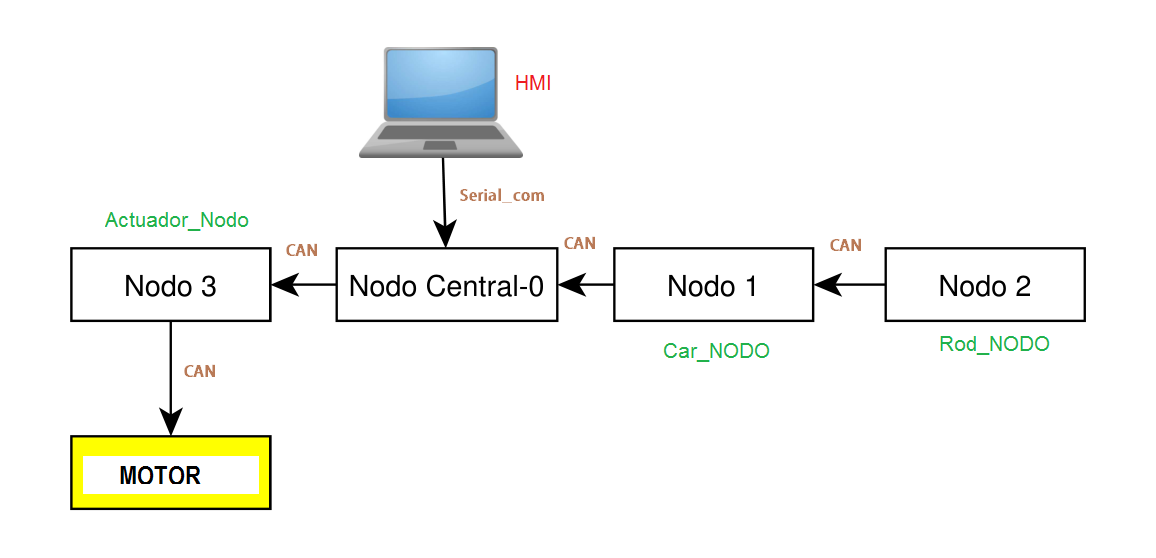
\includegraphics[width=14cm, height=7cm]{diagramacan}
	\caption{Diagrama general de la red}
	\label{fig:diagramacan}
\end{figure}
\end{center}


\subsection{Dise'no l'ogico general  de red}
Se prevee un esquema general de la red con todos sus nodos como se muestra en la Fig. \ref{fig:diagramacan}. Se utiliza el IDE de Arduino para el desarrollo del control de todos los nodos. El nodo primordial es el as'i llamado nodo central o nodo 0.

\begin{figure}[ht]
	\centering
		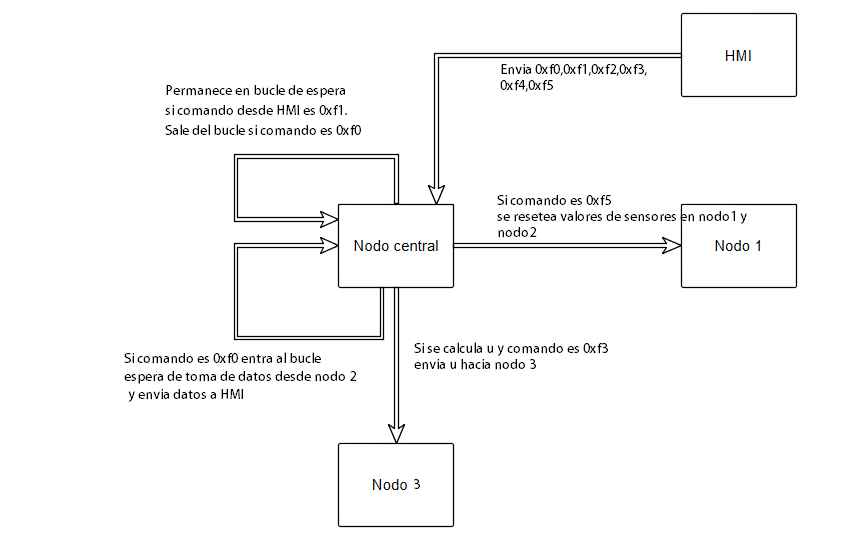
\includegraphics[scale=0.65]{nodocentral}
	\caption{Diagrama de m'aquina de estado del Nodo central}
	\label{fig:nodocentral}
\end{figure}

\subsection{Dise'no l'ogico de la estructura de la red: Nodo 0 }
En est'e nodo se realizar'an las acciones de control en base a la informaci'on proveniente del nodo 2; se encapsular'a la acci'on de control y se enviar'a al nodo 3; tambi'en tendra la importante funci'on de servir de enlace entre la HMI y la red CAN enviando y recibiendo informaci'on desde y hacia la PC, por tanto este nodo es el que m'as carga de trabajo tendr'a, ya que experimentar'a dos tipos de comunicaci'on: CAN y serial y la misi'on de calcular el controlador para el sistema Fig. \ref{fig:nodocentral}.

\subsubsection{Programaci'on nodo 0}

{\tiny
\begin{lstlisting}[language=C]
// demo: CAN-BUS Shield, send data
#include "mcpointer-can.h"
#include <SPI.h>
#include "TimerOne.h"

boolean txOn = false;  // whether the frame is complete
unsigned char counterRx = 0;
unsigned char bufferRx[20] = {0,0,0,0,0,0,0,0,0,0,0,0,0,0,0,0,0,0,0,0};
unsigned char len = 0;
unsigned char buf[8]= {0,0,0,0,0,0,0,0};
float float0 = 0; //numbers to be sent
float float1 = 0;
unsigned char *pointer-float0 = (unsigned char *)&float0;
unsigned char *pointer-float1 = (unsigned char *)&float1;

float float2 = 0; //values of analog read for tests
float float3 = 0;//values of analog read for tests
float float4 = 0; //numbers to be received from HMI
float float5 = 10; //numbers to be received from HMI
unsigned char *pointer-float15 = (unsigned char *)&float5; ////numbers to be received time for sampling (ts)(float)
float float6 = 0; //numbers to be received from HMI
float float7 = 0; //numbers to be received  from HMI
float *pointer-float4 = (float *)&bufferRx[1]; //value of gain
float *pointer-float5 = (float *)&bufferRx[5]; // time sampling (10-50)
float *pointer-float6 = (float *)&bufferRx[1]; // on/off
float *pointer-float7 = (float *)&bufferRx[5]; //tipe of control

//numbers to be received  from CAN
float   float10=0;
float *pointer-float10 = (float *)&buf[0]; //value of Time sampling from CAN

float   float11=0; 
float *pointer-float11 = (float *)&buf[4]; //value of Time sampling from CAN

float dxSensor1[]={0,0};
float dxSensor2[]={0,0};
float  dxres1=0;
float  dxres2=0;
float  rtime;
unsigned char *pointer-dx1 = (unsigned char *)&dxres1;
unsigned char *pointer-dx2 = (unsigned char *)&dxres2;
unsigned char *pointer-rtime = (unsigned char *)&rtime;
int cont2=0;


// the cs pin of the version after v1.1 is default to D9
// v0.9b and v1.0 is default D10
const int SPI_CS_PIN = 10;
const int ledHIGH    = 1;

const int LED=8;
const int LED2=7;
int cont=0;
boolean ledON=1;
unsigned char stmp[8] = {0,0,0,0,0,0,0,0};
unsigned char stmp2[8] = {0,0,0,0,0,0,0,0};
MCpointer-CAN CAN(SPI_CS_PIN);                                    // Set CS pin

void setup()
{
   Timer1.initialize(140000);         // Dispara cada 140 ms
  Timer1.attachInterrupt(ISR_timer); // Activa la interrupcion y la asocia a ISR_Blin
    Serial.begin(115200);

    while (CAN_OK != CAN.begin(CAN_1000KBPS))              // init can bus : baudrate = 500k
    {

    }  
   CAN.sendMsgBuf(0x70,0, 8, stmp);
    
}
void ISR_timer()
   {
    
  unsigned char i; 
  unsigned char eof[4] = {'c','X','r','C'};
  dxSensor1[1]=float2;
  dxSensor2[1]=float3;
  dxres1=(dxSensor1[1]-dxSensor1[0])/float5;
  dxres2=(dxSensor2[1]-dxSensor2[0])/float5;
  
  //this is is for take values of analog in uncomment analog read
  float2=float2;
  float3=float3;
  float0 = float2;
  float1 = float3;
 
  //this is for test if HMI is sending the two first values 4 controls
  
  //float0 = float4;
  //float1 = float5;
  //this is for test if HMI is sending the two first values 4 control
  //float0 = float6;
  //float1 = float7;
  

    //Serial.println(CAN.getCanId());
    digitalWrite(LED,1);
    
  
     //delay(float5);                       // send data 100ms per cycle
     
 
    if (txOn)
  {
   
    for (i=0; i<4; i++)
      //Serial.write(*pointer-float0 + i);
      Serial.write(pointer-float0[i]);


    for (i=0; i<4; i++)
      //Serial.write(*pointer-float1 + i);
      Serial.write(pointer-float1[i]);

      
    for (i=0; i<4; i++)
      Serial.write(pointer-dx1[i]);

      
    for (i=0; i<4; i++)
      Serial.write(pointer-dx2[i]);
    
    for (i=0; i<4; i++)
      Serial.write(pointer-rtime[i]);
      
    for (i=0; i<4; i++)
      Serial.write(eof[i]);
      
   
  }
  
    if(float6==0){
      unsigned char p[4]={0,0,0,0};
      unsigned char e[4] = {'c','X','r','C'};
    for (i=0; i<4; i++)
      //Serial.write(*pointer-float0 + i);
      Serial.write(p[i]);


    for (i=0; i<4; i++)
      //Serial.write(*pointer-float1 + i);
      Serial.write(p[i]);

      
    for (i=0; i<4; i++)
      Serial.write(p[i]);

      
    for (i=0; i<4; i++)
      Serial.write(p[i]);
    
    for (i=0; i<4; i++)
      Serial.write(p[i]);
      
    for (i=0; i<4; i++)
      Serial.write(e[i]);
      
   
    }
  dxSensor1[0]=dxSensor1[1];
  dxSensor2[0]=dxSensor2[1]; 
 
    
    }
void loop()
{  
   interrupts();  
		read();
	rtime = millis(); 
 
}

void read(){
   // unsigned char len = 0;
   // unsigned char buf[8];
    
    if(CAN_MSGAVAIL == CAN.checkReceive())            // check if data coming
    {
      CAN.readMsgBuf(&len, buf);    // read data,  len: data length, buf: data buf
      unsigned char canId = CAN.getCanId();
       
      if(CAN.getCanId()==0x20){    
       float10=(*pointer-float10);
       float11=(*pointer-float11);
       // if(float5>=10){
       // CAN.sendMsgBuf(0x70,0, 8, stmp);
       // }

       float2=float10;
		u = -gain1*cartPos - gain2*cartVel - gain3*rodPos - gain4*rodVel + gain5*error;
    }
    digitalWrite(LED,1);
  }
  else{
     
      if(float6==1){
        CAN.sendMsgBuf(0x70,0, 8, stmp);
        CAN.sendMsgBuf(0x10,0, 8, stmp2);
        }
     }
  
   digitalWrite(LED,1);
   
}
int aux=0;
void serialEvent()
{
  digitalWrite(LED2,0);
 
  while (Serial.available())
  {
    
   digitalWrite(LED2,1);
    bufferRx[counterRx] = (unsigned char)Serial.read(); //get the new byte
    
    if (counterRx >= 8)
    {
      counterRx = 0;
       
       
      switch (bufferRx[0]) //analyze command on first byte
      {
        case 0xf0:
          txOn = true;
//          here make a union of bytes to build the float registers
     
          float4 = (*pointer-float4);
          float5 = (*pointer-float5);  
   //here we send the value of ts from HMI to CAN
          stmp[0] = pointer-float15[0];
          stmp[1] = pointer-float15[1];
          stmp[2] = pointer-float15[2];
          stmp[3] = pointer-float15[3];
          
            aux+=1;
        break;
        case 0xf2:
          txOn = true;
//          here make a union of bytes to build the float registers        
          float6 = (*pointer-float6);
          float7 = (*pointer-float7);  
          aux+=1;      
        break;   
        case 0xf1:
          txOn = false;
          aux=0;
        break;
      } 
    }
    else
      counterRx++;  
    }   
 }

 \end{lstlisting}
}

\subsubsection{Controlador implementado en el nodo 0}
'Este es el controlador del sistema implementado en el nodo 0.
{\footnotesize
\begin{lstlisting}[language=C]
u = -gain1*cartPos - gain2*cartVel - gain3*rodPos - gain4*rodVel + gain5*error;

 \end{lstlisting}
}



\subsubsection{Sistema el'ectrico del nodo 0}

A continuaci'on se detalla el sistema de conexi'on del sistema el'ectrico del nodo 0 en la Fig. \ref{fig:nodo0electric}:
\begin{center}
\begin{figure}[ht]
	\centering
		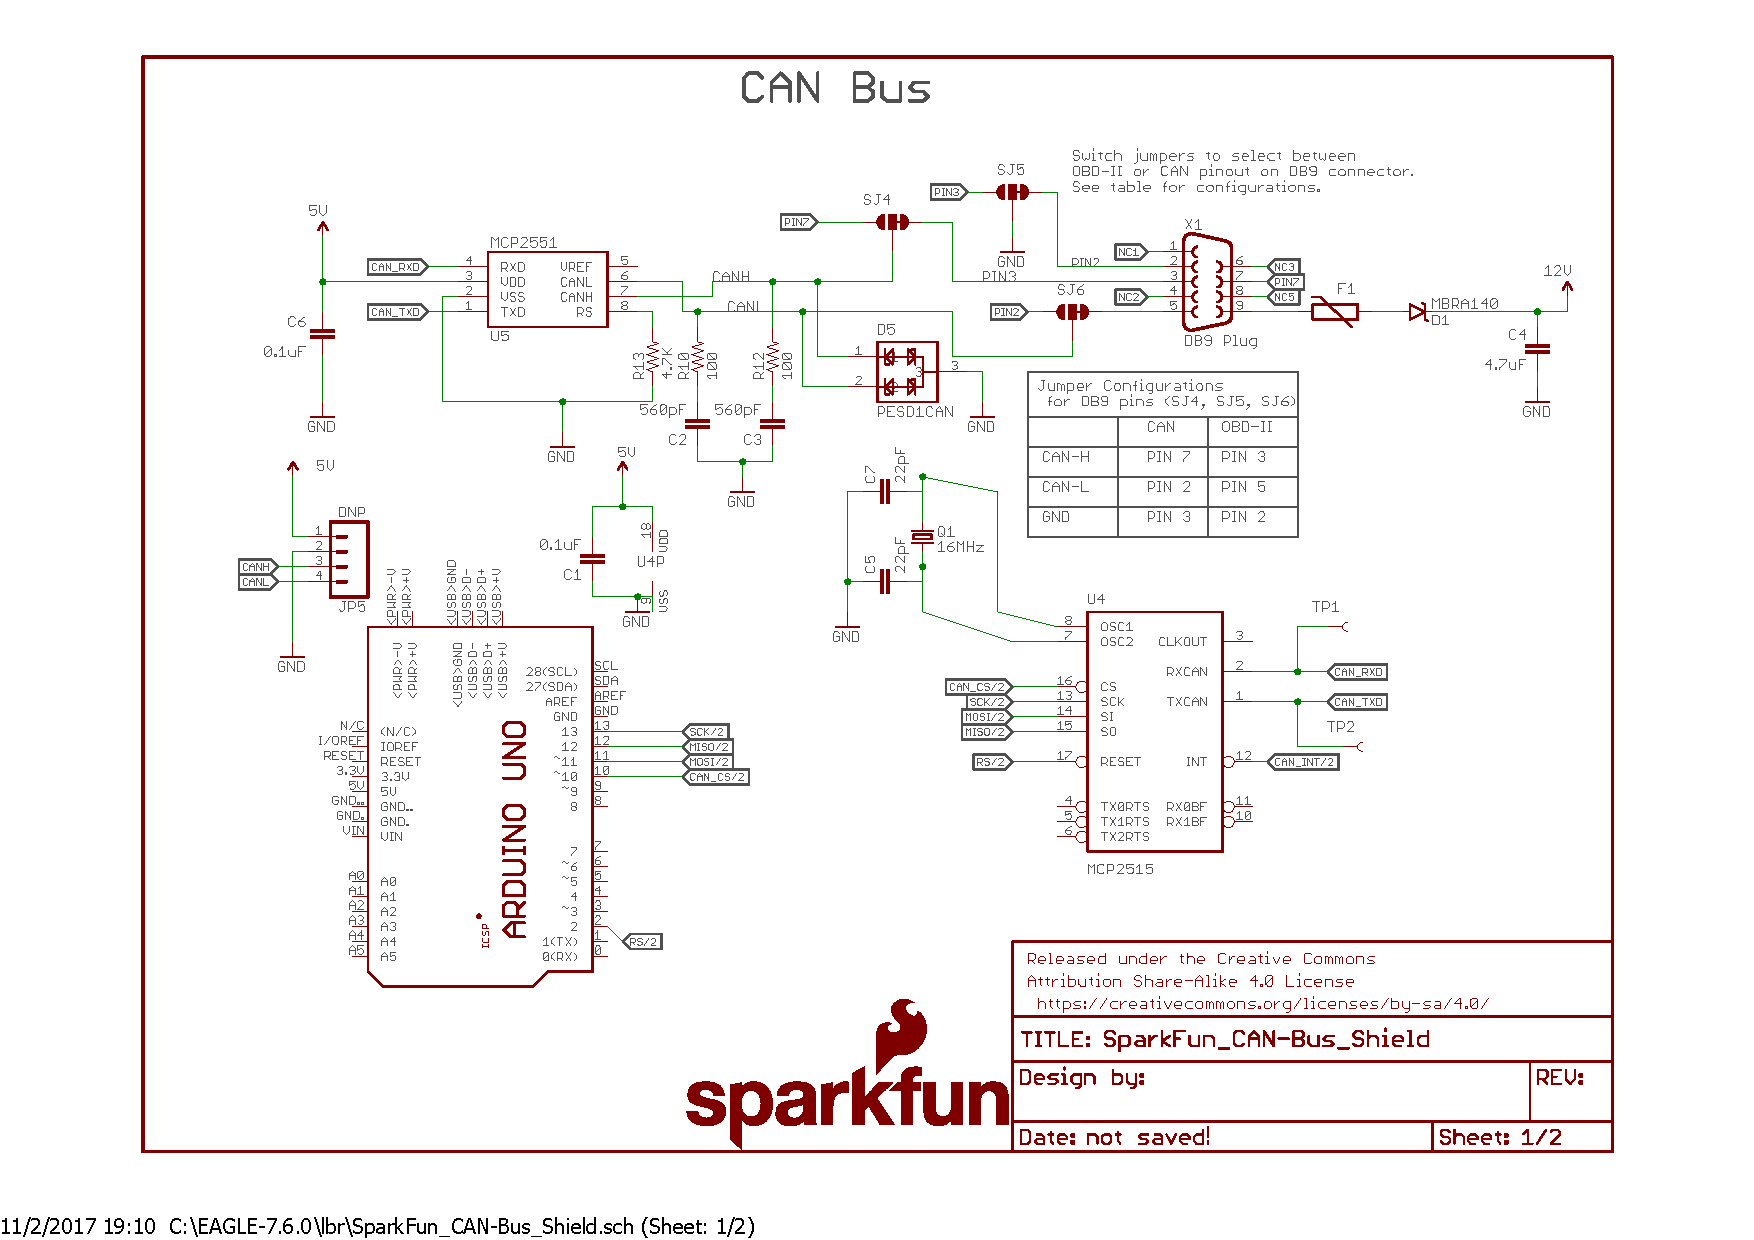
\includegraphics[width=14cm, height=10cm]{nodo0elec}
	\caption{Diagrama el'ectrico del nodo 0}
	\label{fig:nodo0electric}
\end{figure}
\end{center}

\subsection{Dise'no l'ogico de la estructura de la red: Nodo 1}

\subsubsection{M'aquina de estado Nodo 1}
En est'e nodo estar'a conectado el sensor ubicado en el motor con una particularidad, en este nodo se disparar'a las alarmas la toma de datos del sensor cada time sampling (ts) especificado en la HMI, que tendr'a que ser enviada primero al nodo central y luego a 'este; por defecto el nodo tiene un sampling de 10 (ms), siendo el rango permitido desde 10ms hasta 50 ms. En 'este nodo s'olomente se toman datos y se envian al nodo 2 como se muestra en la Fig. \ref{fig:nodo1}.Todas las librerias usadas se encuentran disponibles en la p'agina oficial de Arduino o en su defecto en la de terceros.
\begin{figure}[ht]
	\centering
		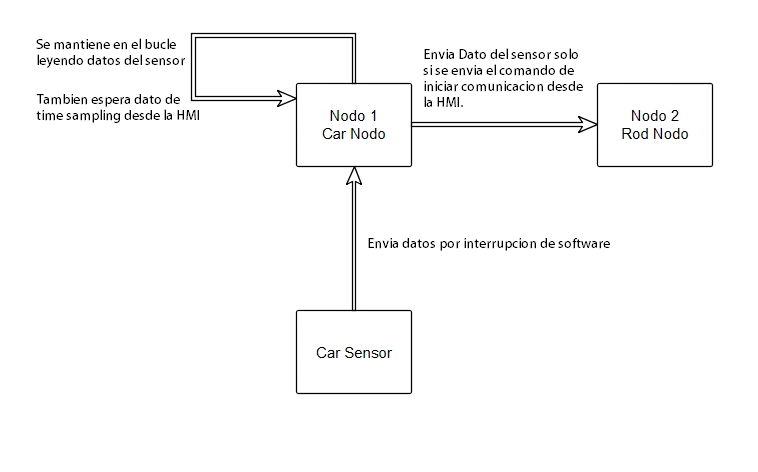
\includegraphics[scale=0.6]{nodo1}
	\caption{M'aquina de estado del Nodo 1}
	\label{fig:nodo1}
\end{figure}
\subsubsection{Programaci'on nodo 1}

Para el envio de datos se hace un direccionamiento indirecto; a continuaci'on toda la programaci'on: 

{\tiny

\begin{lstlisting}[language=C]

#include <SPI.h>
#include "mcpointer-can.h"
#include <Encoder.h>
#include <Timer.h>

Encoder myEnc(5, 6);
// the cs pin of the version after v1.1 is default to D9
// v0.9b and v1.0 is default D10
const int SPI_CS_PIN = 10;
const int LED=8;
unsigned char len = 0;
unsigned char buf[8]= {0,0,0,0,0,0,0,0};
boolean ledON=1;
float   float0=0;
unsigned char *pointer-float0 = (unsigned char *)&float0; //
unsigned long   float1=10; //this value never be less than 10 ms
unsigned long float2=10;

float *pointer-float1 = (float *)&buf[0]; //value of Time sampling from Central Controller 
int   aux=0;
float   aux2=0;
float   aux3=0;
float   aux4=0;
//int aux5=10;

Timer t;

unsigned char stmp[8] = {0, 0, 0, 0, 0, 0, 0, 0};
MCpointer-CAN CAN(SPI_CS_PIN);                                    // Set CS pin

void setup()
{
  //Timer1.initialize(10000);         // Dispara cada 10 ms
//  Timer1.attachInterrupt(ISR_timer); // Activa la interrupcion y la asocia a ISR_Blin
interrupts();
int tickEvent = t.every(float1, ISR_timer );   
    Serial.begin(115200);
    pinMode(LED,OUTPUT);
  
    while (CAN_OK != CAN.begin(CAN_1000KBPS))              // init can bus : baudrate = 500k
    {
       Serial.println("CAN BUS Shield init fail");
       Serial.println(" Init CAN BUS Shield again");
       // delay(100);
    }
    Serial.println("CAN BUS Shield init ok!");
    
}
void loop()
{
   
  int tickEvent = t.every(float1, ISR_timer );  
 // Timer1.stop();
 
 float0= myEnc.read();
  t.update();
  read(); 
 // delay(10);
 
}
void ISR_timer()
   {
    //float0= myEnc.read();
    
      Serial.println(float0);
      Serial.println(float1);
     //Serial.println(float1);
     //Serial.println(float2);
     //Serial.println(float3);
    
    
      //Timer1.restart();
    
  
  //  Serial.println(float2);

        stmp[0]= pointer-float0[0];
        stmp[1]= pointer-float0[1];
        stmp[2]=pointer-float0[2];
        stmp[3]=pointer-float0[3];
        CAN.sendMsgBuf(0x60,0, 8, stmp);    
   //Serial.println(float0);
    //Serial.println(float2);

   }
void read(){
   //unsigned char len = 0;
   // unsigned char buf[8];

    if(CAN_MSGAVAIL == CAN.checkReceive())            // check if data coming
    {
      CAN.readMsgBuf(&len, buf);    // read data,  len: data length, buf: data buf
      unsigned char canId = CAN.getCanId();
      // Serial.println(CAN.getCanId());
      if(CAN.getCanId()==0x70){
       
        float1=(*pointer-float1); //add to float1 the value of the pointer from de CAN buffer (time sampling).
        
         
         if(float1<=10) float1=10;
         if(float1>=50) float1=50;
         
         if(float2!=float1){
         
         Serial.println("TIme sampling has changed");
         }
         float2=float1;
    
    }
     digitalWrite(LED,1);
  }
  
  }

/*********************************************************************************************************
  END FILE
*********************************************************************************************************/

\end{lstlisting}
}
\subsubsection{Sistema el'ectrico del nodo 1}

A continuaci'on se detalla el sistema de conexi'on del sistema el'ectrico del nodo 1 en la Fig. \ref{fig:nodo1electric}:

\begin{center}
\begin{figure}[ht]
	\centering
		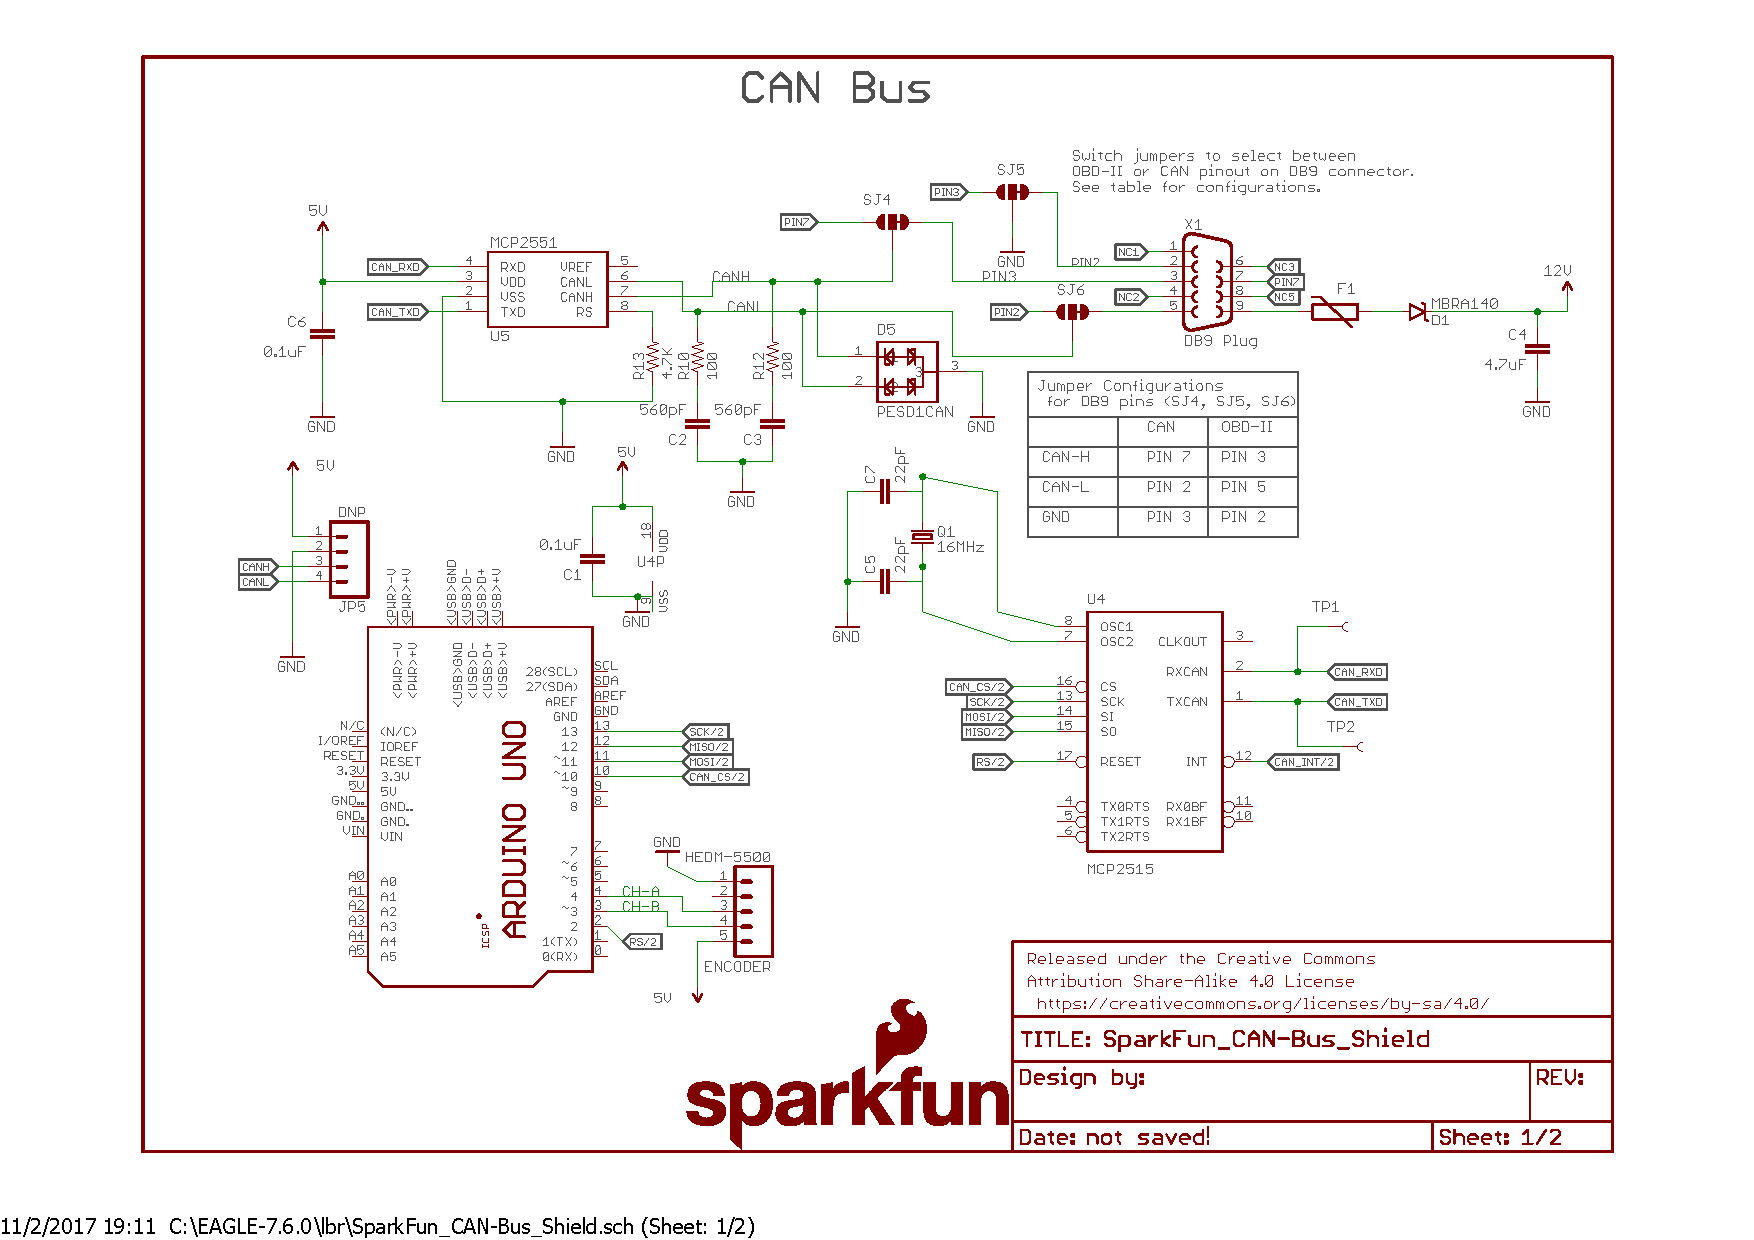
\includegraphics[width=14cm, height=10cm]{nodo1elec}
	\caption{Diagrama el'ectrico del nodo 1}
	\label{fig:nodo1electric}
\end{figure}
\end{center}

\subsection{Dise'no l'ogico de la estructura de la red: Nodo 2}

\subsubsection{M'aquina de estado del Nodo 2}
En este nodo se toman datos del sensor ubicado en el p'endulo con una particularidad; s'olo se disparar'a el envio de datos al nodo central cada vez que le llegue informaci'on del nodo 1; luego 'este tomar'a el dato del sensor, lo encapsular'a, lo pondr'a en la cola a continuaci'on de los datos del nodo 1 que pasan directamente de la entrada a la salida del buffer de la red y enviar'a ambos datos al nodo central, como se muestra en la Fig. \ref{fig:nodo2}.


\begin{figure}[ht]
	\centering
		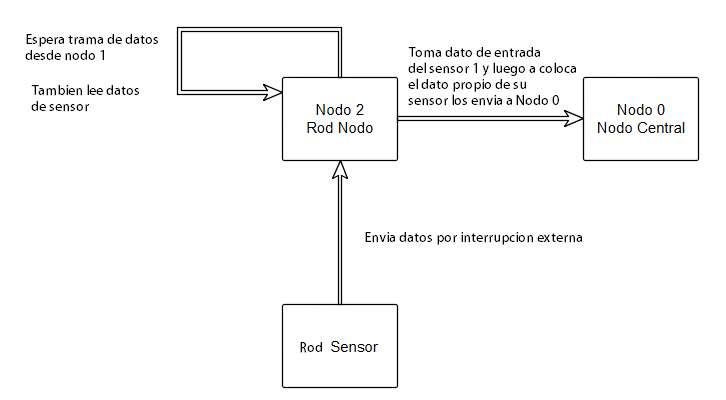
\includegraphics[scale=0.6]{nodo2}
	\caption{M'aquina de estado del Nodo 2}
	\label{fig:nodo2}
\end{figure}

\subsubsection{Programaci'on nodo 2}

Para el envio de datos se hace direccionamiento indirecto de datos; se crean dos variables de clase CAN para guardar el dato de entrada y luego ponerlo en el buffer de salida.
{\tiny
\begin{lstlisting}[language=C]

#include <SPI.h>
#include "mcpointer-can.h"
#include <Encoder.h>
Encoder myEnc(5, 6);
// the cs pin of the version after v1.1 is default to D9
// v0.9b and v1.0 is default D10
const int SPI_CS_PIN = 10;
const int LED=8;
unsigned char len = 0;
unsigned char buf[8]= {0,0,0,0,0,0,0,0};
float   float0=0;
unsigned char *pointer-float0 = (unsigned char *)&float0;
int   aux=0;
float   aux2=0;
 float u=0;
  float v=0;
   float w=0;
   int z=0;
unsigned char stmp[8] = {0, 0, 0, 0, 0, 0, 0, 0};

float   float10=0; //keep the data from the arduino w sensor 1
float *pointer-float10 = (float *)&buf[0]; //value

MCpointer-CAN CAN(SPI_CS_PIN);                                    // Set CS pin

void setup()
{
    Serial.begin(115200);
    pinMode(LED,OUTPUT);

    while (CAN_OK != CAN.begin(CAN_1000KBPS))              // init can bus : baudrate = 500k
    {
        //Serial.println("CAN BUS Shield init fail");
     //   Serial.println(" Init CAN BUS Shield again");
      }
    //Serial.println("CAN BUS Shield init ok!");
}
void loop()
{
  float0=  myEnc.read(); 
  read();  
}

void read(){
    if(CAN_MSGAVAIL == CAN.checkReceive())            // check if data coming
    {
      CAN.readMsgBuf(&len, buf);    // read data,  len: data length, buf: data buf
      unsigned char canId = CAN.getCanId();
       //Serial.println(CAN.getCanId());
      if(CAN.getCanId()==0x60){
           
        float10=(*pointer-float10);
       
        Serial.println(float0);
         
        // v=(buf[0]+(buf[1]*3.917647)/1000);
         //u=(buf[2]*3.917647)/1000;
         //z=v*100;
        //w=(1.00*z/100)+((u/100));
        //w=v+((u/1000));
        stmp[0]= buf[0];
        stmp[1]= buf[1];
        stmp[2]= buf[2];
        stmp[3]= buf[3];
        //stmp[3]= float0;
        stmp[4]= pointer-float0[0];
        stmp[5]= pointer-float0[1];
        stmp[6]= pointer-float0[2];
        stmp[7]= pointer-float0[3];
        CAN.sendMsgBuf(0x20,0, 8, stmp);  
        
            digitalWrite(LED,1);
       
    }           
    digitalWrite(LED,1);
  }  
  }

\end{lstlisting}
}
\subsubsection{Sistema el'ectrico del nodo 2}

La Fig. \ref{fig:nodo1electric}, muestra la conexi'on a utilizarse en el nodo 2, la cual es similar al nodo 1.
\subsection{Dise'no l'ogico de la estructura de la red: Nodo 3}
\subsubsection{M'aquina de estados del Nodo 3}
\begin{figure}[ht]
	\centering
		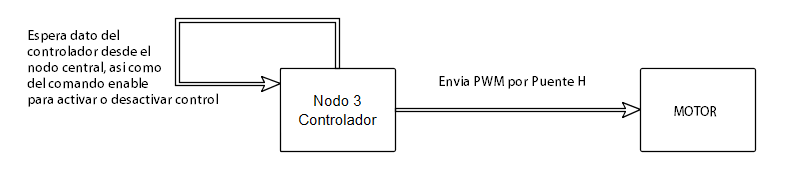
\includegraphics[scale=0.65]{nodo3}
	\caption{M'aquina de estados del Nodo 3}
	\label{fig:nodo3}
\end{figure}

\subsubsection{Nodo del motor: Nodo 3 }
En este nodo se pone en evidencia las acciones enviadas por el controlador central (Fig. \ref{fig:nodo3}).

\subsubsection{Programaci'on nodo 3}

{\tiny
\begin{lstlisting}[language=C]

#include <SPI.h>
#include "mcpointer-can.h"

// the cs pin of the version after v1.1 is default to D9
// v0.9b and v1.0 is default D10
const int SPI_CS_PIN = 10;
const int LED=8;
float   aux2=0;
boolean ledON=1;
unsigned char stmp[8] = {0, 0, 0, 0, 0, 0, 0, 0};
MCpointer-CAN CAN(SPI_CS_PIN);                                    // Set CS pin

void setup()
{
    Serial.begin(115200);
    pinMode(LED,OUTPUT);

    while (CAN_OK != CAN.begin(CAN_1000KBPS))              // init can bus : baudrate = 500k
    {
        Serial.println("CAN BUS Shield init fail");
        Serial.println(" Init CAN BUS Shield again");
        
    }
    Serial.println("CAN BUS Shield init ok!");
}
void loop()
{
  read();   
}

void read(){
  unsigned char len = 0;
    unsigned char buf[8];

    if(CAN_MSGAVAIL == CAN.checkReceive())            // check if data coming
    {
      CAN.readMsgBuf(&len, buf);    // read data,  len: data length, buf: data buf
      unsigned char canId = CAN.getCanId();
       //Serial.println(CAN.getCanId());
      if(CAN.getCanId()==0x10){

        Serial.println("-----------------------------");
        Serial.println("get data from ID: ");
        Serial.println(canId);

        for(int i = 0; i<len; i++)    // print the data
        {
            Serial.print(buf[i]);
            Serial.print("\t");
            
             if(!buf[0])
            {

                digitalWrite(LED,1);
                ledON=1;
            }
        }
        Serial.println();     
    }           
  }
  }

/*********************************************************************************************************
  END FILE
*********************************************************************************************************/
 \end{lstlisting}
}


\subsubsection{Sistema esquem'atico el'ectrico del nodo 3}

A continuaci'on se detalla el sistema de conexi'on del sistema el'ectrico del nodo 0 en la Fig. \ref{fig:nodo3electric}:

\begin{center}
\begin{figure}[ht]
	\centering
		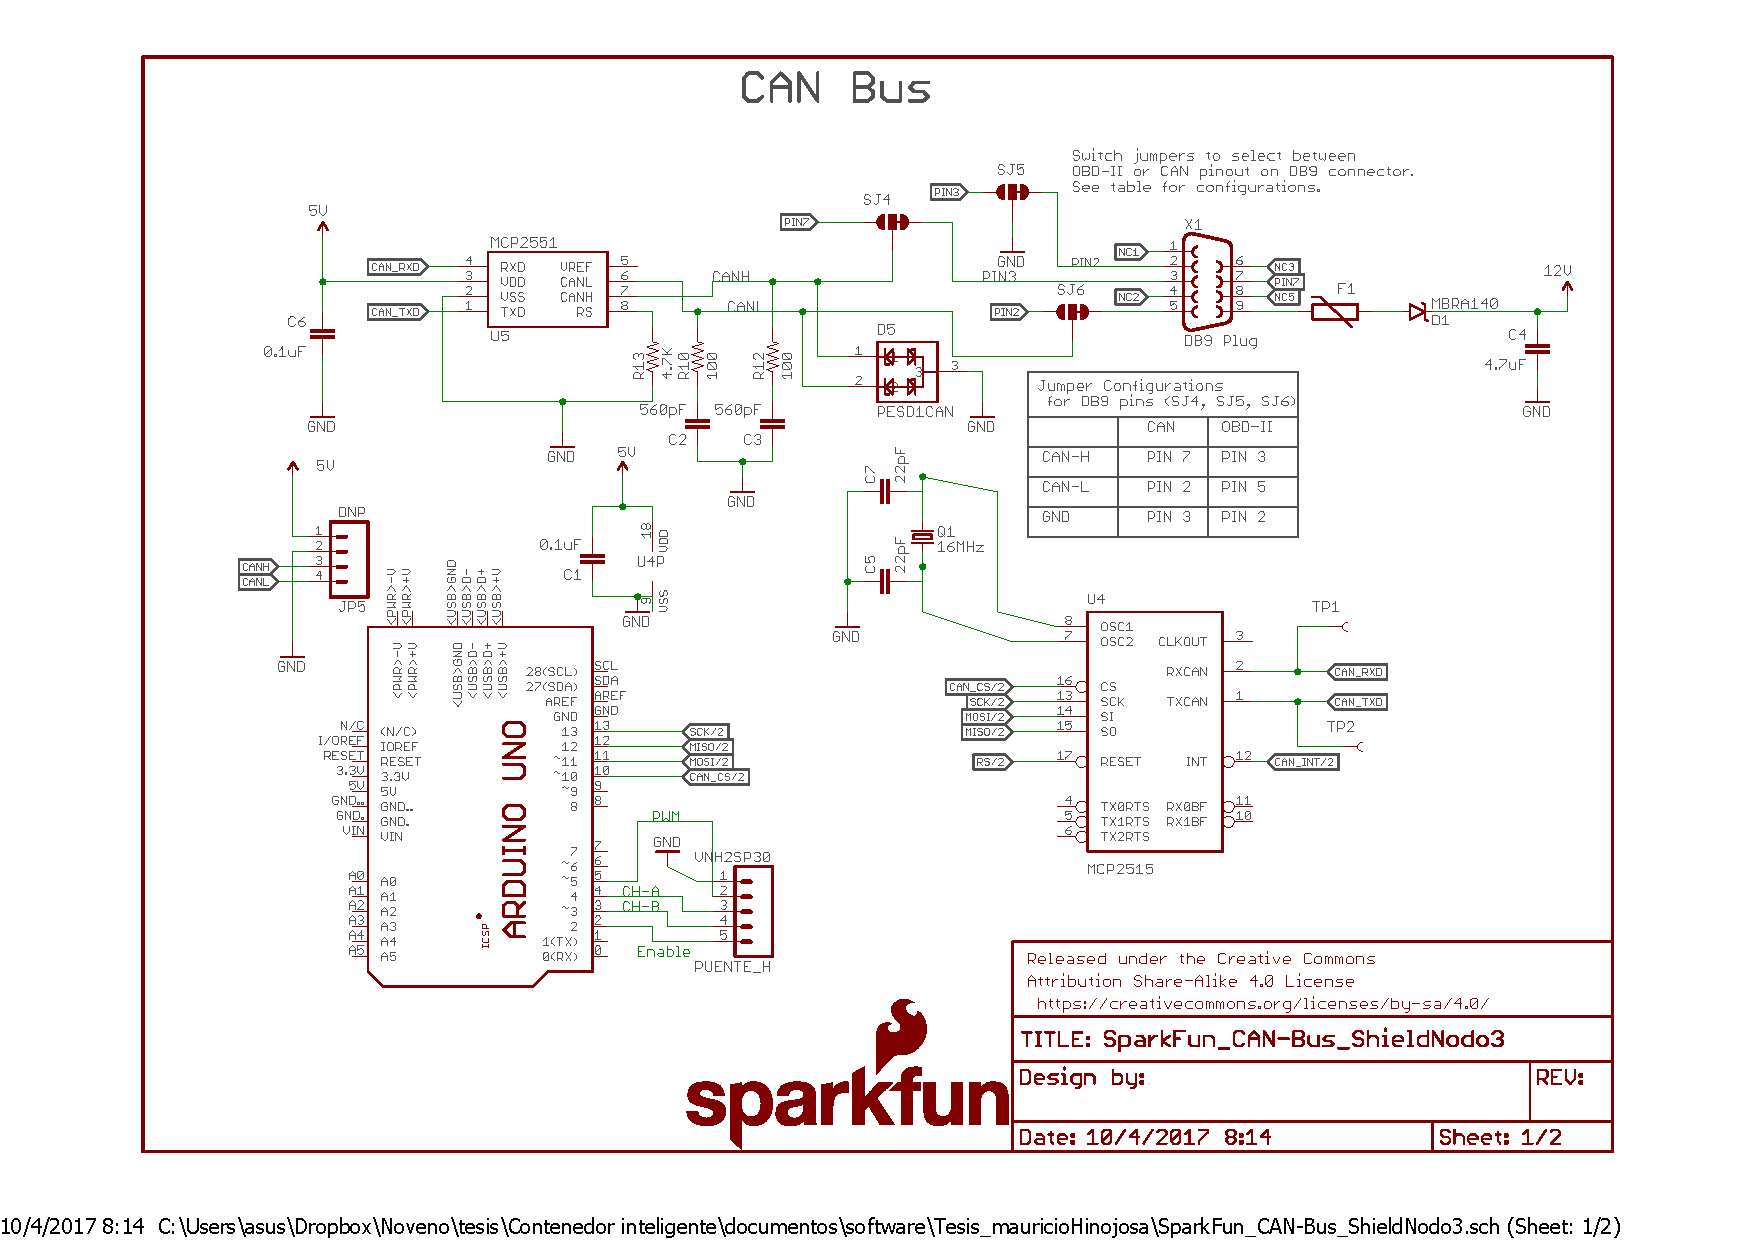
\includegraphics[width=14cm, height=10cm]{nodo3e}
	\caption{Diagrama el'ectrico del nodo 3}
	\label{fig:nodo3electric}
\end{figure}
\end{center}

\subsection{Red f'isica CAN e interconexi'on con la HMI}

En esta secci'on se muestra la interconexi'on de la red CAN y la HMI, as'i como de los sensores implementados en la red; el puente H de electr'onica del sistema como se muestra en la Fig.\ref{fig:canhmi}.
\begin{center}
\begin{figure}[ht]
	\centering
		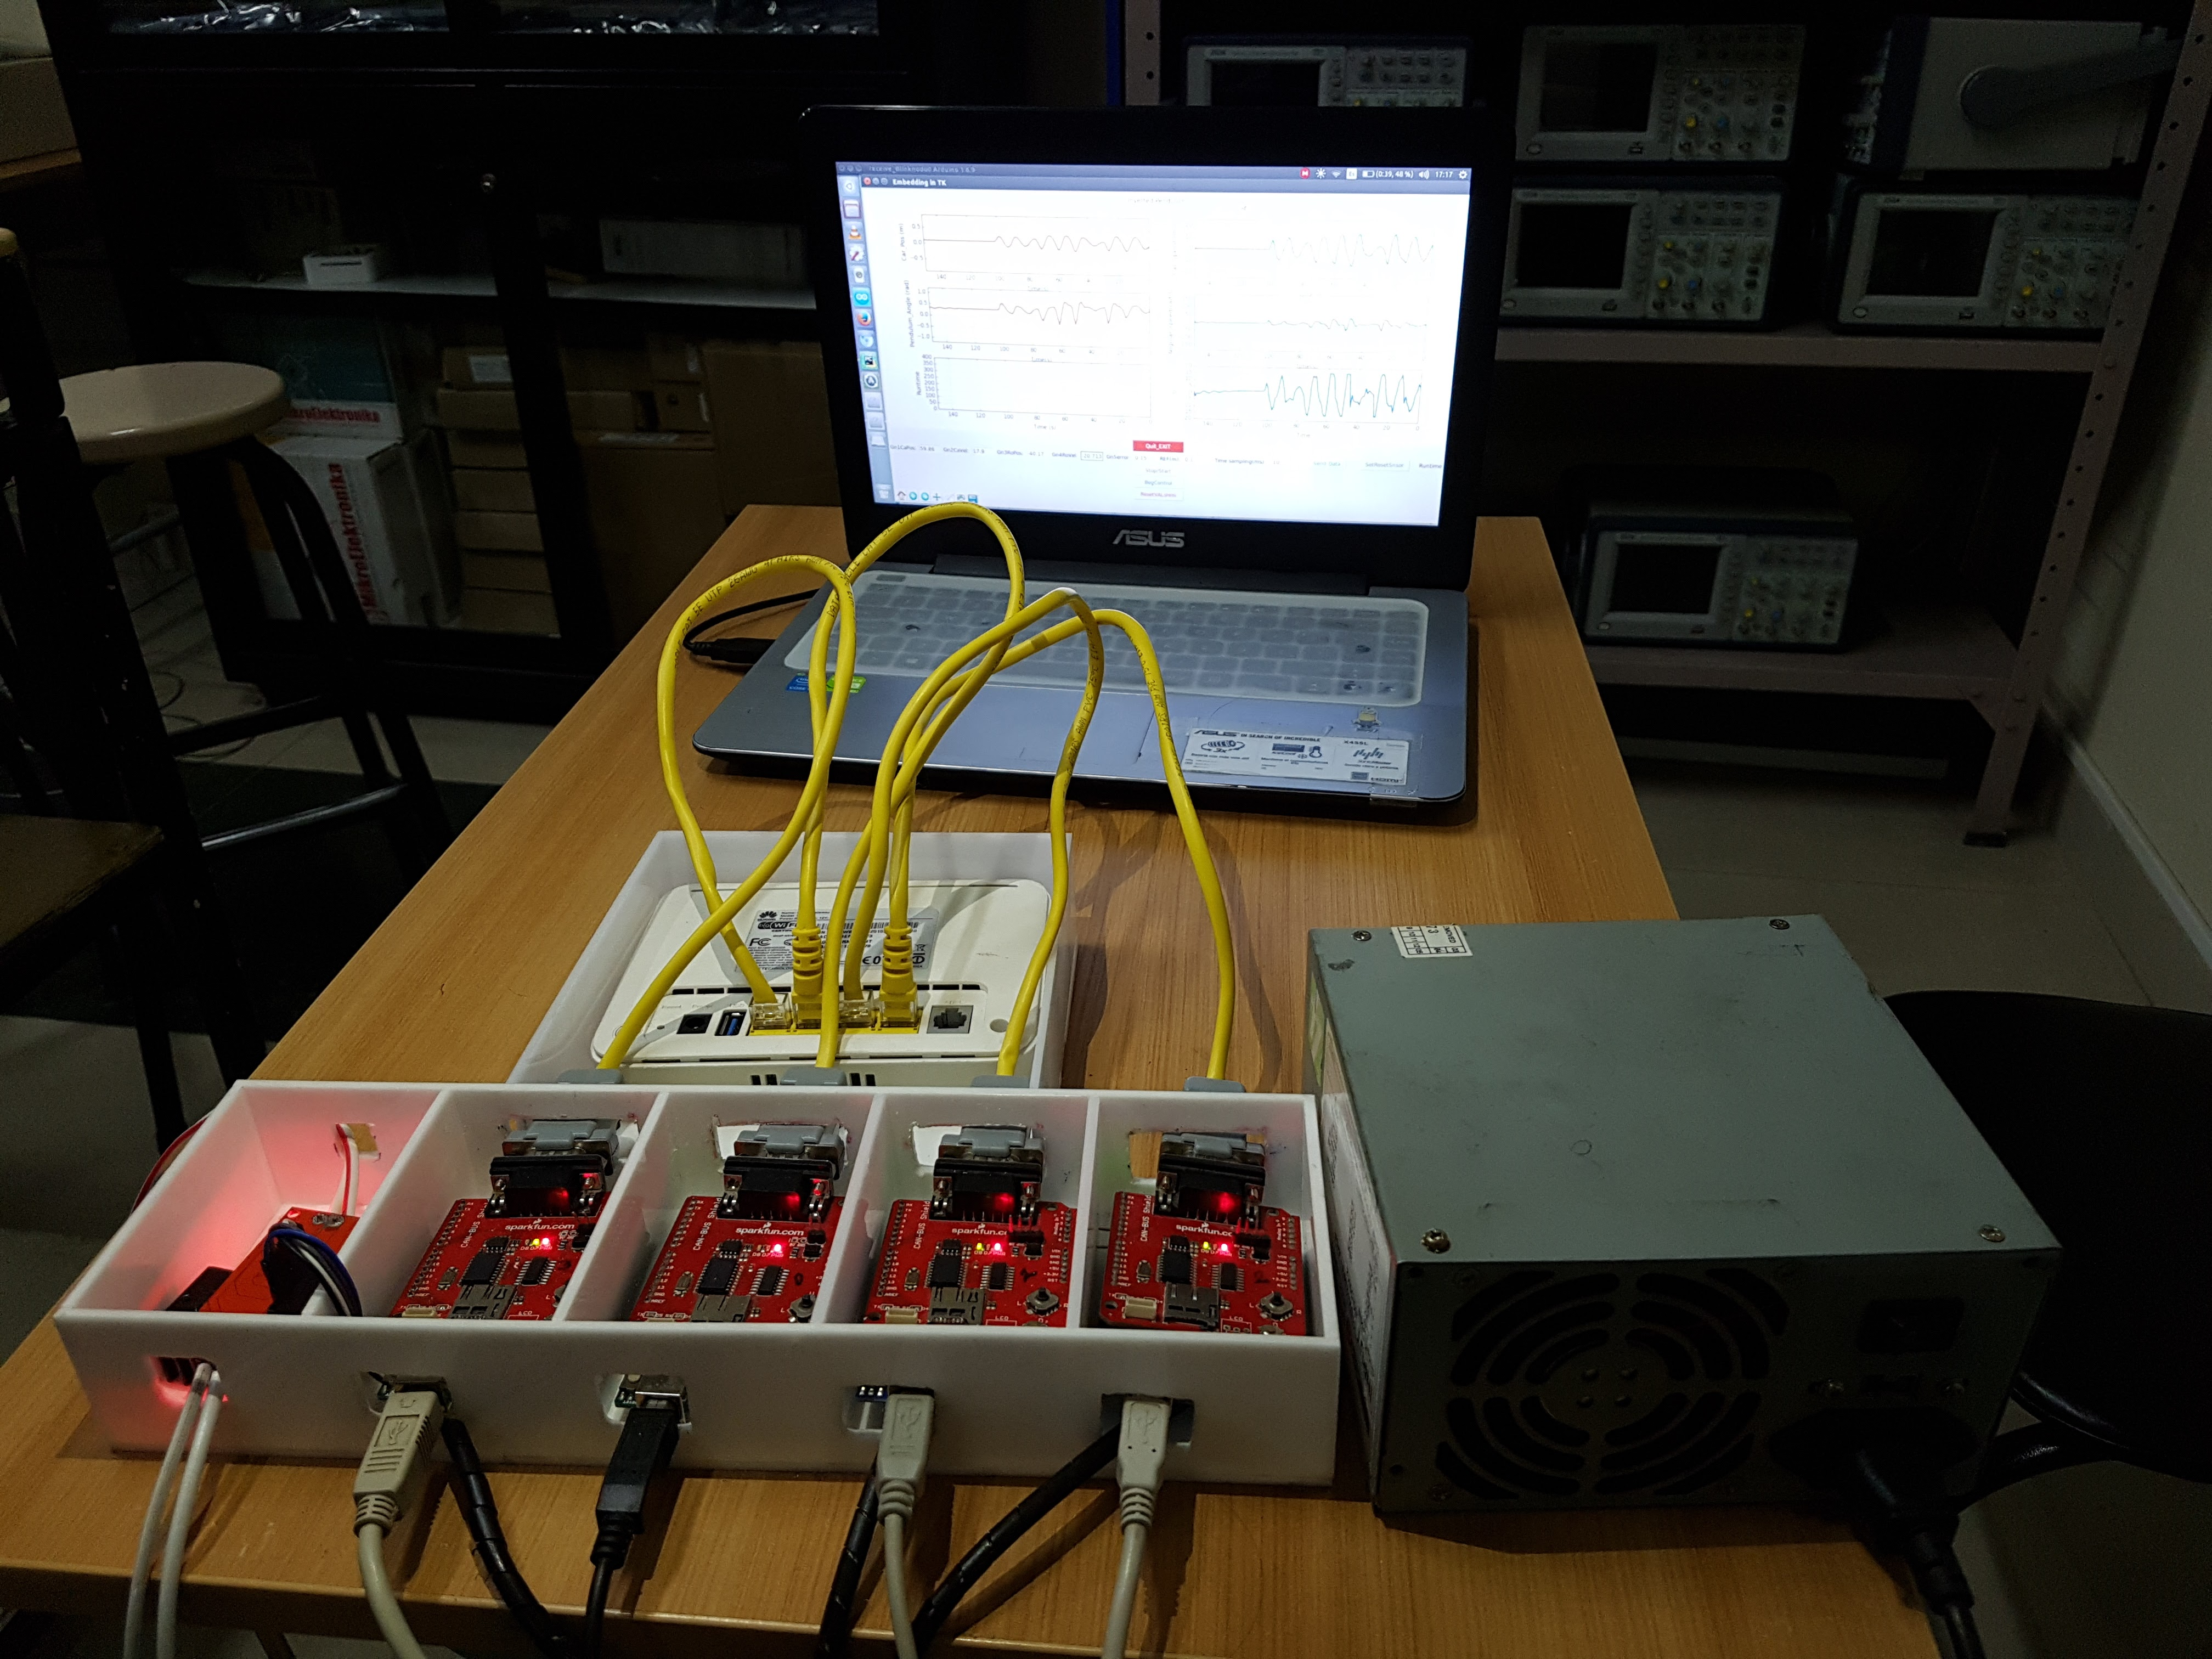
\includegraphics[width=14cm, height=10cm]{canhmi}
	\caption{CAN y HMI}
	\label{fig:canhmi}
\end{figure}
\end{center}


\section{Dise'no de la HMI}
\subsection{Instalaci'on de Python en Ubuntu}
La instalaci'on de Python dentro de Ubuntu no tiene ninguna complicaci'on:
\begin{itemize}
	\item Se debe abrir una terminal \textbf{(Ctrl $+$ Alt $+$ t)}.
	\item Con la correspondiente conexi'on a internet y  se debe escribir en consola lo siguiente:
	
	\begin{itemize}
		\item {\small
\begin{lstlisting}[language=C]
sudo add-apt-repository ppa:fkrull/deadsnakes
\end{lstlisting}
}

		\item {\small
\begin{lstlisting}[language=C]
sudo apt-get update
\end{lstlisting}
}
		\item {\small
\begin{lstlisting}[language=C]
sudo apt-get install python2.7
\end{lstlisting}
}
	\end{itemize}
	\item Por ultimo: {\small\begin{lstlisting}[language=C]
	sudo apt-get update \end{lstlisting}}
	{\small\begin{lstlisting}[language=C]
	sudo apt-get upgrade \end{lstlisting}} y todo estar'a listo para ejecutar Python.
\end{itemize}

\subsection{Instalaci'on de PyCharm}
PyCharm es un IDE, que tiene una version paga y una versi'on (community) de libre de desarrollo la cual ser'a implementada para el desarrollo del sistema HMI, y utiliza como estructructura y lenguaje de desarrollo el antes instalado Python 2.7.2, entre algunos otros lenguajes; y contiene varias herramientas de desarrollo, como ya se explico en secciones anteriores.
La instalaci'on de PyCharm dentro de Ubuntu no tiene ninguna complicaci'on:
\begin{itemize}
	\item Se debe abrir una terminal.
	\item Con la correspondiente conexi'on a internet y escribir en la consola lo siguiente:
	
	\begin{itemize}
		\item {\small
\begin{lstlisting}[language=C]
sudo add-apt-repository ppa:mystic-mirage/pycharm
\end{lstlisting}
}

		\item {\small
\begin{lstlisting}[language=C]
sudo apt-get update
\end{lstlisting}
}
		\item {\small
\begin{lstlisting}[language=C]
sudo apt-get install pycharm-community
\end{lstlisting}
}
	\end{itemize}
	\item Por ultimo se hace un : {\small\begin{lstlisting}[language=C]
	sudo apt-get update \end{lstlisting}}
	{\small\begin{lstlisting}[language=C]
	sudo apt-get upgrade \end{lstlisting}} y todo estar'a listo para ejecutar Python.
\end{itemize}



\subsection{Desarrollo del software}

EL desarrollo del software de supervisi'on de la HMI, parti'o de un software b'asico de intercambio de informaci'on con un Arduino programado en lenguaje \textbf{Python 2.7.2} mostrado en los anexos; en el que el programa se envia dos datos y el arduino respond'ia devolviendo los mismos datos cada cierto tiempo, para graficarlos en la HMI. Basados en esta premisa  se tuvo principalmente tres etapas de desarrollo: expansi'on el buffer del puerto Usb para el env'io de datos, desarrollo de los sistemas gr'aficos y de procesamiento de informaci'on y el desarrollo de controles para el HMI.

\subsection{Expansi'on el buffer del puerto Usb}

Al principio la informaci'on que se enviaba desde la HMI era de un dos datos por el buffer de salida de la HMI; a lo cual se procedi'o a expandirlo hasta que se puedan enviar los datos necesarios para el control desde la HMI final, dando como resultado 10 datos o 40 bytes de informaci'on a la targeta de Arduino que corresponde al nodo 0 o controlador central conectado por Usb a la Pc.


\subsection{Desarrollo de los sistemas gr'aficos y de procesamiento de informaci'on }
Se contaba con una s'ola gr'afica implementada en el programa origen, de la cual se parti'o para conseguir 6 gr'aficas, de las que la primera representa la posici'on del sensor del carro, en la segunda muestra la velocidad de cambio de posici'on del carro; la tercera datos de posici'on del sensor del p'endulo; en la cuarta se regresenta la variaci'on de velocidad del sensor pendular; la quinta el tiempo de procesamiento que lleva el nodo 0 desde su arranque en microsegundos y la sexta representa el controlador.

\subsection{Procesamiento de informaci'on y el desarrollo de controles}

B'asicamente se implentementaron todo tipo de herramientas que permiten desde la creaci'on de botones, cuadros de texto, modificadores gr'aficos  que permiten la manipulaci'on externa de la HMI; hasta la creaci'on de variables que guardan informaci'on o se utilizan para el envio y recepci'on de datos; las clases y objetos que permiten manipular la HMI internamente; librer'ias especiales como la de la Usb o la librer'ia para el empaquetado de datos (todas las librer'ias incluidas en el IDE tool de Python); as'i como como las estructuras l'ogicas o matem'aticas necesarias para el desarrollo; logo de PyCharm en la Fig. \ref{fig:pycharm}
\begin{figure}[ht]
	\centering
		
\includegraphics[scale=0.4]{pycharm}
	\caption{Logo identificativo de Pycharm}
	\label{fig:pycharm}
\end{figure}


\subsection{Programaci'on de la HMI en Python}
A continuaci'on se muestra la programaci'on realizada en Python para la HMI.
\\
 {\tiny
\begin{lstlisting}[language=python]
#!/usr/bin/env python
# -*- coding: utf-8 -*-
"""
@authors: carlos xavier rosero
          manel velasco garc'ia
          Maurico Hinojosa Rea
best performance tested with python 2.7.3, GCC 2.6.3, pyserial 2.5
"""

from __future__ import division
import serial  #serial commun library
import struct  #library to reestructure bytes on buffer
import time #time for delay library
from collections import deque #library for structure of data
import matplotlib
matplotlib.use('TkAgg')
from matplotlib.backends.backend_tkagg import FigureCanvasTkAgg, NavigationToolbar2TkAgg
# implement the default mpl key bindings
from matplotlib.backend_bases import key_press_handler
from matplotlib.pyplot import Figure
import matplotlib.animation as animation #library for plotting
import matplotlib.pyplot as plt #library for plotting
from matplotlib.widgets import Slider, Button, RadioButtons
from Tkinter import *
import sys
if sys.version_info[0] < 3:
    import Tkinter as Tk
else:
    import tkinter as Tk
import os #library native

class puerto:
    puerto0='/dev/ttyACM0'
    j=0
    j=1
    i=0
#########################################
# ###########################################################
##########################################                       ###################################
##########################################  VENTANA DE Puertos ###################################
##########################################                       ###################################
####################################################################################################

class AllTkinterWidgets:
    def __init__(self, master):
        frame = Tk.Frame(master, width=500, height=400, bd=1)
        frame.pack()

        iframe1 = Tk.Frame(frame, bd=2, relief=SUNKEN)

        def closeall():

            master.quit()  # stops mainloop
            master.destroy()
            puerto.j=2

        def closewindow():

            master.quit()  # stops mainloop
            master.destroy()


        def selectbutton():
            puerto.j=1
            k = v.get()
            puerto.puerto0 = k
            print k
            print puerto.puerto0


        Tk.Button(iframe1, text='CloseAll', fg="red",
				command=closeall).pack(side=LEFT, padx=5)
        Tk.Button(iframe1, text='Done', fg="blue",
				command=closewindow).pack(side=LEFT, padx=5)
        Tk.Button(iframe1, text='Select Port',fg="green",
				command=selectbutton).pack(side=LEFT, padx=5)
        #Tk.Checkbutton(iframe1,
				#text='CheckButton').pack(side=LEFT, padx=5)

        v = StringVar()

        a=Tk.Radiobutton(iframe1, text='/dev/ttyACM5', variable=v,
                    value='/dev/ttyACM5').pack(side=RIGHT, anchor=W)
        b=Tk.Radiobutton(iframe1, text='/dev/ttyACM4', variable=v,
                    value='/dev/ttyACM4').pack(side=RIGHT, anchor=W)

        c=Tk.Radiobutton(iframe1, text='/dev/ttyACM3', variable=v,
                    value='/dev/ttyACM3').pack(side=RIGHT, anchor=W)

        d=Tk.Radiobutton(iframe1, text='/dev/ttyACM2', variable=v,
                    value='/dev/ttyACM2').pack(side=RIGHT, anchor=W)

        e=Tk.Radiobutton(iframe1, text='/dev/ttyACM1', variable=v,
                    value='/dev/ttyACM1').pack(side=RIGHT, anchor=W)
        f=Tk.Radiobutton(iframe1, text='/dev/ttyACM0', variable=v,
                       value='/dev/ttyACM0').pack(side=RIGHT, anchor=W)
        iframe1.pack(expand=1, fill=X, pady=10, padx=5)


root = Tk.Tk()
# root.option_add('*font', ('verdana', 10, 'bold'))
all = AllTkinterWidgets(root)
root.title('Port Selection')
root.mainloop()

#########################################
# ###########################################################
##########################################                       ###################################
##########################################  VENTANA DE MONITOREO ###################################
##########################################                       ###################################
####################################################################################################

class command:
    startCx = 0xf0  #startcx value for comunication
    startCx2 = 0xf2  #startcx value for comunication 2
    stopCx = 0xf1   #stopcx value for comunication


class cons:

    #######################################
    ###### here we create global variables#####
    #######################################

    div=1
    max1=0
    runtime1=float(0)
    k=float(0)
    ts=float(50)
    onoff=float(1)
    typecontroll=float(1)





# use this part only with old versions of python and libraries
# tested specifically with python 2.6.5, GCC 4.4.3, serial 1.3.5
class adapt(serial.Serial):
    def write(self, data):
        super(self.__class__, self).write(str(data))

#################################################

class serialCx:

    def __init__(self, usbPort, frameLen, maxLen, EOL, bauds):
        #SELF (VARIABLES for the _init_ class)
        self.ay1 = deque([0.0] * maxLen)
        self.ay2 = deque([0.0] * maxLen)
        self.ay3 = deque([0.0] * maxLen)
        self.ay4 = deque([0.0] * maxLen)
        self.ay5 = deque([0.0] * maxLen)
        self.maxLen = maxLen
        self.eol = EOL  # end of line
        self.lenEol = len(self.eol)  # length of the end of line
        self.frameLen = frameLen - self.lenEol
        self.float0 = float(0) #var analog1
        self.float1 = float(0) #var analog2
        self.valor1 = float(0) #var analog1 dy/dt
        self.valor2 = float(0) #var analog2 dy/dt
        self.runtime = float(0)  # var analog2 dy/dt
                            #this all var are going to the plot
        # open serial port
        self.ser = adapt(port=usbPort,
				baudrate=bauds, timeout=1, parity=serial.PARITY_NONE,
                         stopbits=serial.STOPBITS_ONE)

        #######################################
        ######here we send initial values to the arduino0 #####
        #######################################

        #self.ser.open
        #self.ser.isOpen
        time.sleep(2)  # waits until arduino gets up
        inputS = []  # initializes buffer
        while self.ser.inWaiting() > 0:  # neglects the trash code received
            inputS.append(self.ser.read(1))  # appends a new value into the buffer

        self.float0ToTx = cons.k  # initial values of the floating
				#numbers to be sent--------> value of k gain
        self.float1ToTx = cons.ts # initial values of the floating
				#numbers to be sent--------> value of ts (tme sampling) 10-50 ms
        self.float2ToTx = cons.onoff  # initial values of the floating 
				#numbers to be sent--------> on/of arduino's communication
        self.float3ToTx = cons.typecontroll  # initial values of the floating 
				#numbers to be sent--------> Tipe of controller crank/inverted

        cons.div=self.float1ToTx
        value0 = struct.pack('%sf' % 1, self.float0ToTx)  # splits the float value into 4 strings
        value1 = struct.pack('%sf' % 1, self.float1ToTx)  # splits the float value into 4 strings
        value2 = struct.pack('%sf' % 1, self.float2ToTx)  # splits the float value into 4 strings
        value3 = struct.pack('%sf' % 1, self.float3ToTx)  # splits the float value into 4 strings

        time.sleep(0.2) #this wait before buffer finish write
        # this buffer sends the command to start tx from arduino and both floating registers
        buffer = bytearray([command.startCx,
				ord(value0[0]), ord(value0[1]), ord(value0[2]), ord(value0[3]),
        ord(value1[0]), ord(value1[1]), ord(value1[2]), ord(value1[3])])

        self.ser.write(buffer)  # sends the command to start the reception

        time.sleep(0.075) #this wait before buffer finish write

        buffer = bytearray([command.startCx2,
				ord(value2[0]), ord(value2[1]), ord(value2[2]), ord(value2[3]),
        ord(value3[0]), ord(value3[1]), ord(value3[2]), ord(value3[3])])
        self.ser.write(buffer)  # sends the command to start the reception
        # add to buffer
        time.sleep(0.1)  # this wait before buffer finish write


    def addToBuf(self, buf, val):
        if len(buf) < self.maxLen:
            buf.append(val)
        else:
            buf.pop()
            buf.appendleft(val)


    # update plot
    def update(self, frameNum, a1, a2, a3, a4,rtime):

        #######################################
        ######here we get the data from the buffer for update on plots #####
        #######################################

        line = bytearray()
        try:
            while True:
                c = self.ser.read(1)
                if c:
                    line.append(c)
                    if line[-self.lenEol:] == self.eol:  # verifies if EOF has been received
                        line = line[0:-self.lenEol]  # removes EOF
                        break
                else:
                    break

            if len(line) == self.frameLen:
                self.float0 = struct.unpack('f', line[0:4])
                self.float0 = self.float0[0]  # takes out the only one element from the tuple
                self.float1 = struct.unpack('f', line[4:8])
                self.float1 = self.float1[0]  # takes out the only one element from the tuple
                self.valor1 = struct.unpack('f', line[8:12])
                self.valor1=self.valor1[0]   # takes out the only one element from the tuple
                self.valor2 = struct.unpack('f', line[12:16])
                self.valor2 = self.valor2[0]  # takes out the only one element from the tuple
                self.runtime = struct.unpack('f', line[16:20])
                self.runtime = self.runtime[0]   # takes out the only one element from the tuple

                print self.float0, #coma ad a espace on the plot window
                print self.float1,
                print self.valor1,
                print self.valor2,
                print self.runtime,
                print cons.ts,
                print cons.k,
                print cons.onoff,
                print cons.typecontroll
                cons.max1 = self.valor1
                cons.runtime1=self.runtime

                # add data to buffer
                self.addToBuf(self.ay1, self.float0)
                self.addToBuf(self.ay2, self.float1)
                self.addToBuf(self.ay3, self.valor1)
                self.addToBuf(self.ay4, self.valor2)
                self.addToBuf(self.ay5, self.runtime)
                a1.set_data(range(self.maxLen), self.ay1)
                a2.set_data(range(self.maxLen), self.ay2)
                a3.set_data(range(self.maxLen), self.ay3)
                a4.set_data(range(self.maxLen), self.ay4)
                rtime.set_data(range(self.maxLen), self.ay5)
            else:
                print 'Incorrect frame length:',
                print self.float0,  # coma ad a espace on the plot window
                print self.float1,
                print self.valor1,
                print self.valor2,
                print self.runtime
                print self.frameLen
                print len(line)
                #self.ser.write(buffer)
                #self.ser.flushInput()  # gets empty the serial port buffer


        except KeyboardInterrupt:
            print('Exiting...')

    def printrtime(self):
        print self.runtime
        return self.runtime
    # clean up
    def close(self):
        # close serial

        buffer = bytearray([command.stopCx, 0x01, 0x01, 0x01, 0x01, 0x01, 0x01,
                            0x01, 0x01])  # the (0x01) is used only to fill the buffer
        # in order to accomplish the standard length

        self.ser.write(buffer)  # sends the command to start the reception

        self.ser.flushInput()
        self.ser.close()




def plotting(givenData):


    #######################################
    ###### here we create the variables for canvas and plt #####
    #######################################

    root = Tk.Tk()
    root.wm_title("Embedding in TK")
    #f = plt.figure(figsize=(9, 6), dpi=95, facecolor = 'w', edgecolor = 'k')
    fig = plt.figure(num = 1, figsize = (9, 5.5),
		dpi = 95, facecolor = 'w', edgecolor = 'k') #modifie plot's properties


    #######################################
    ######this are just propierties of plt and sub plt#####
    #######################################

    plt.rc('lines', linewidth=1.2) #modifie weigh of lines
    plt.rc('font', size=10) # modifie weight of text
    plt.suptitle('Inverted Pendulum')# add subplot title
    plt.subplots_adjust(hspace=0.30)



    #######################################
    ###### here we can change properties from each subplots #####
    #######################################

    #ax1 =  f.add_subplot(111)
    ax1 = plt.subplot(321)
    ax1.grid(True)
    a1, = ax1.plot([0], [0], color=(0, 1, 1)) ##comma means continuous plotting
    plt.xlim(0, 150)
    plt.ylim(-2500, 2500)

    plt.xlim(plt.xlim()[::-1])
    plt.ylabel('Analog1')
    plt.xlabel('Time')
    plt.grid(color = 'r', linewidth = 1)
    #plt.legend(loc=2)
    plt.title('', fontsize=20, color='0.5', verticalalignment=
		'baseline', horizontalalignment='center')

    ax2 = plt.subplot(323)
    ax2.grid(True)
    a2, = ax2.plot([0], [0], color=(1, 1, 0))
    plt.xlim(0, 150)
    plt.ylim(-2500, 2500)
    plt.xlim(plt.xlim()[::-1])#invert x axe's direction if
		#this line is disable plotting change direction
    plt.ylabel('Analog2')
    plt.xlabel('Time')
    plt.grid(color = 'b', linewidth = 1)
    plt.title(' ', fontsize=20, color='0.5', verticalalignment='baseline', 
		horizontalalignment='center')

    ax3 = plt.subplot(322)
    ax3.grid(True)
    a3, = ax3.plot([0], [0], color=(0, 1, 0))
    plt.xlim(0, 15)
    plt.ylim(-50, 50)  # modifie limits on y axis
    plt.xlim(plt.xlim()[::-1])  # invert x axe's direction
    plt.ylabel('Derivative1')
    plt.xlabel('Time')
    plt.grid(color='m', linewidth=1)
    plt.title(' ', fontsize=20, color='0.5', verticalalignment='baseline', 
		horizontalalignment='center')

    ax4 = plt.subplot(324) #_first num add y subplots _second_num add
		#x subplot _3_num put in the correct place the subplot
    ax4.grid(True)#this add grid on subplot
    a4, = ax4.plot([0], [0], color=(0, 0, 1)) #
    #a3, = ax4.plot([0], [0], color=(0, 1, 0)) #unline to plot two lines in the same plot
    plt.xlim(0, 15) #modifie limits on x axis
    plt.ylim(-50, 50) #modifie limits on y axis
    plt.xlim(plt.xlim()[::1])  # invert x axe's direction

    plt.ylabel('Derivative2') #this add ylabel title
    plt.xlabel('Time') #this add xlabel title
    plt.grid(color='y', linewidth=1) #modifie properties of the grid
    plt.title(' ', fontsize=20, color='0.5', 
		verticalalignment='baseline', horizontalalignment=
		'center')#modifie title's properties on subplots

    ax5 = plt.subplot(325) #_first num add y subplots _second_num add 
		#x subplot _3_num put in the correct place the subplot
    ax5.grid(True)#this add grid on subplot
    rtime, = ax5.plot([0], [0], color=(0, 0, 1)) #

    plt.xlim(0, 50) #modifie limits on x axis
    plt.ylim(0, 100000) #modifie limits on y axis
    plt.xlim(plt.xlim()[::-1])  # invert x axe's direction
    plt.ylabel('runtime') #this add ylabel title
    plt.xlabel('Time') #this add xlabel title
    plt.grid(color='g', linewidth=1) #modifie properties of the grid
    plt.title(' ', fontsize=20, color='0.5',
		verticalalignment='baseline', horizontalalignment=
		'center')#modifie title's properties on subplots
    plt.subplots_adjust(left=0.1)
    plt.subplots_adjust(right=0.95)
   # selection2 = str(cons.runtime1)
   # label3.config(text=selection2)
    #anim = animation.FuncAnimation(f, 
		givenData.update, fargs=(a1, a2, a3, a4, rtime),frames=1000, interval=1) 
		#update values on plot #200 frames each 1 ms

    anim = animation.FuncAnimation(fig,
		givenData.update, fargs=(a1, a2, a3, a4, rtime), frames=1000,interval=1)  
		# update values on plot #200 frames each 1 ms

    #######################################
    ######bottons inside canvas #####
    #######################################


    #here we made the canvas for the bottons and other things
    ###############################################
    canvas = FigureCanvasTkAgg(fig, master=root)
    canvas.show()
    canvas.get_tk_widget().pack(side=Tk.TOP, fill=Tk.BOTH, expand=1)

    toolbar = NavigationToolbar2TkAgg(canvas, root)
    toolbar.update()
    canvas._tkcanvas.pack(side=Tk.TOP, fill=Tk.BOTH, expand=1)

    def on_key_event(event):
        print('you pressed %s' % event.key)
        key_press_handler(event, canvas, toolbar)

    canvas.mpl_connect('key_press_event', on_key_event)

    def _quit():
        root.quit()  # stops mainloop
        root.destroy()  # this is necessary on Windows to prevent
        # Fatal Python Error: PyEval_RestoreThread: NULL tstate
    def reset():
         cons.runtime1 = float(0)
         cons.k = float(0)
         cons.ts = float(50)
         cons.onoff = float(1)
         cons.typecontroll = float(1)
         print cons.runtime1,cons.typecontroll,cons.onoff, cons.ts, cons.k
         serialCx(puerto.puerto0, 24, 300, 'cXrC',
                     115200)# Fatal Python Error: PyEval_RestoreThread: NULL tstate

    buttonreset = Tk.Button(master=root, text='Reset', command=reset,fg="red",width=14)
    buttonreset.pack(side=Tk.BOTTOM)
    button = Tk.Button(master=root, text='Quit', command=_quit, fg="red", width=14)
    button.pack(side=Tk.TOP)

    label = Tk.Label(master=root, text="                   ")
    label.pack(side=Tk.LEFT, padx=4)

    labelgain = Tk.Label(master=root, text="Gain : (x.xx)")
    labelgain.pack(side=Tk.LEFT,padx=4)
    e = Tk.Entry(master=root,width=10)
    e.insert(0,0)
    e.pack(side=Tk.LEFT,padx=20)
    e.focus_set()
    labelts = Tk.Label(master=root, text="Time sampling : (x)")
    labelts.pack(side=Tk.LEFT,padx=4)
    f = Tk.Entry(master=root,width=10)
    f.insert(0,10)
    f.pack(side=Tk.LEFT,padx=35)

    #e.focus_set()

    label = Tk.Label(master=root, text="        ")
    label.pack(side=Tk.LEFT)


    def selectcontrolbutton():
        cons.typecontroll = v.get()
        print v.get()
        print cons.typecontroll

    buttoncontrol = Tk.Button(master=root, text='Type Control',
		command=selectcontrolbutton, fg="purple", width=14)
    buttoncontrol.pack(side=Tk.LEFT)
    rootframe=Tk.Frame(root, bd=1, relief=SUNKEN)
    v = IntVar()
    c = Tk.Radiobutton(rootframe, text='Control1', variable=v,
                       value=1).pack(side=TOP)
    d = Tk.Radiobutton(rootframe, text='Control2', variable=v,
                       value=2).pack(side=TOP)
    t = Tk.Radiobutton(rootframe, text='Control3', variable=v,
                       value=3).pack(side=TOP)
    r = Tk.Radiobutton(rootframe, text='Control4', variable=v,
                       value=4).pack(side=TOP)

    rootframe.pack(side=Tk.LEFT,fill=X)

    label = Tk.Label(master=root, text="          ")
    label.pack(side=Tk.LEFT)



    def changevalbutton():
        k = e.get()
        l = f.get()
        cons.k=float(k)
        cons.ts = int(l)
        print k,l,cons.ts,cons.k
        serialCx(puerto.puerto0, 24, 300, 'cXrC',
                                115200)  # This values modifie serialport, 
		  	#Length of bytes in tx,Length of data plotting, and bauds
        print k, l, cons.ts, cons.k


    def stopcanbutton():

        if puerto.i==1:
            cons.onoff=1
            puerto.i=0
        else:
            cons.onoff = 0
            puerto.i = 1
        print cons.onoff
        serialCx(puerto.puerto0, 24, 300,
				        'cXrC',
                 115200) 
			# This values modifie serialport, 
      #Length of bytes in tx,Length of data plotting, and bauds

        print cons.onoff
        print puerto.i

    b3 = Tk.Button(master=root, text="Send Data", command=changevalbutton, fg="green")
    b3.pack(side=Tk.LEFT,pady=10,padx=10)

    label = Tk.Label(master=root, text="          ")
    label.pack(side=Tk.LEFT)

    b4 = Tk.Button(master=root, text="Stop/Start CAN COM", command=stopcanbutton)
    b4.pack(side=Tk.BOTTOM, pady=10)


    labelruntime = Tk.Label(master=root,text="Runtime")
    labelruntime.pack(side=Tk.LEFT,pady=10)
    label = Tk.Label(master=root, text="    ")
    label.pack(side=Tk.LEFT)
    def runtimebutton():
        s = cons.runtime1
        labelruntime.config(text=s)

    b2 = Tk.Button(master=root, text="Runtime", command=runtimebutton, fg="blue")
    b2.pack(side=Tk.LEFT,pady=10)
    label = Tk.Label(master=root, text="      ")
    label.pack(side=Tk.LEFT)

    #    b2 = Tk.Button(master=root, text="runtime", command=runtimebutton)
 #   b2.pack(side=Tk.RIGHT)




    #######################################
    ######update data from plt from pyplot#####
    #######################################

    #here the plt or figure is updating
    anim = animation.FuncAnimation(fig, givenData.update, fargs=(a1, a2, a3, a4, rtime), frames=1000,
                                   interval=1)  # update values on plot #200 frames each 1 ms
    #plt.show()
    Tk.mainloop()


   # plt.close()
    #plt.show()

    #Tk.mainloop()


#######################################
######here starts the main program#####
#######################################


if __name__ == "__main__":

    testMauricio = serialCx(puerto.puerto0, 24, 300, 'cXrC', 115200) #This values modifie serialport, 
		#Length of bytes in tx,Length of data plotting, and bauds
    if puerto.j==1:
        plotting(testMauricio) #plotting
    serialCx.close(testMauricio) #close all process


\end{lstlisting}

}


\subsection{Ventana HMI terminada}

Concluida la programaci'on se tienen dos ventanas; la primera es una peque'na ventana que permite seleccionar entre diferentes puertos Usb, posibles en Ubuntu  como muestra la Fig. \ref{fig:usb}.
\begin{figure}[ht]
	\centering
		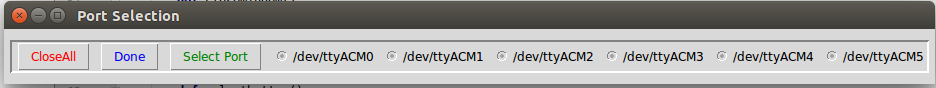
\includegraphics[scale=0.6]{usb}
	\caption{Ventana de selecci'on Usb}
	\label{fig:usb}
\end{figure}
\begin{figure}[ht]
	\centering
		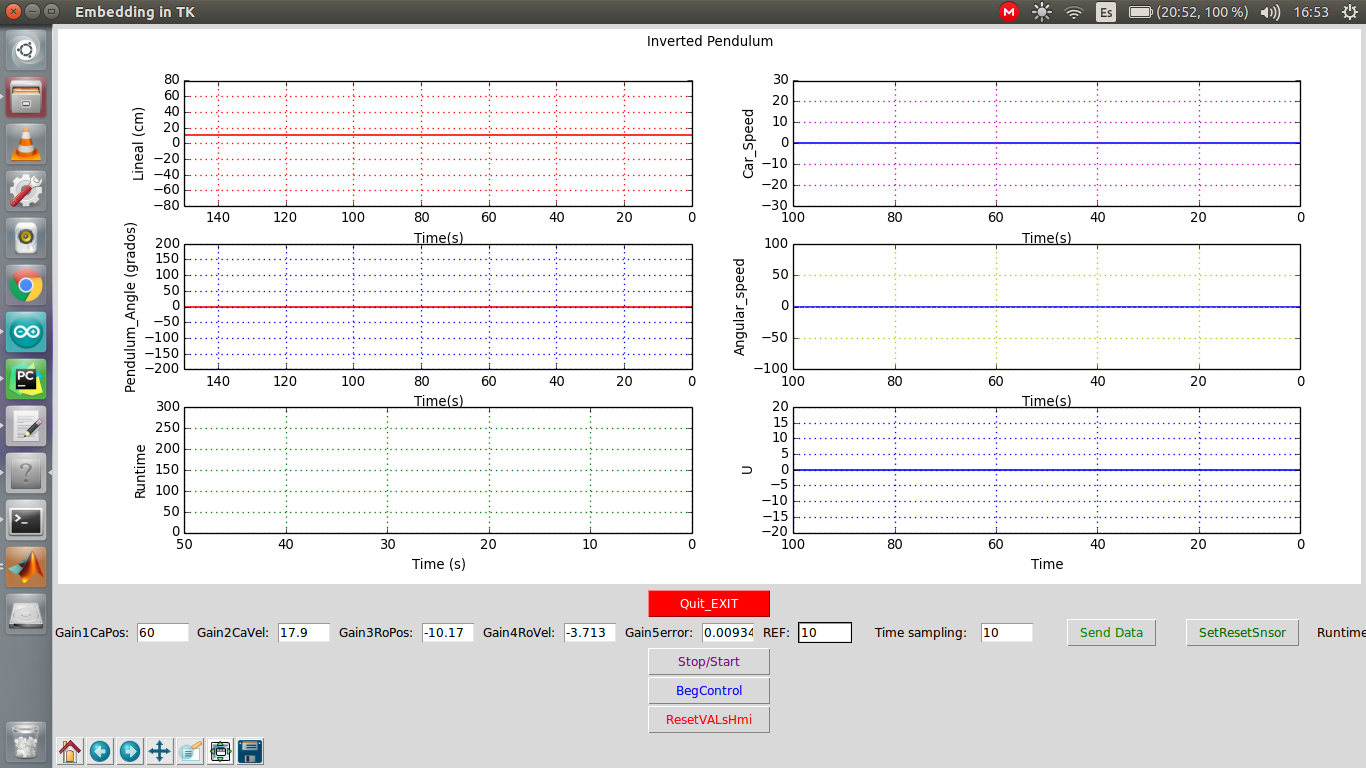
\includegraphics[scale=0.45]{HMI}
	\caption{HMI}
	\label{fig:HMI}
\end{figure}

La segunda ventana es la HMI utilizar en el sistema como muestra Fig. \ref{fig:HMI}, consta de las partes:

\begin{enumerate}
	\item Gr'afica sensor 1.
	\item Gr'afica de la variaci'on de velocidad sensor 1.
	\item Gr'afica sensor 2.
	\item Gr'afica de la variaci'on de velocidad sensor 2.
	\item Gr'afica del tiempo de procesamiento en microsegundos.
	\item Botones y texto de informaci'on y modificaci'on de los valores de control del p'endulo.
	\item Barra de manipulaci'on de las gr'aficas.
\end{enumerate}


\section{Tr'amas de datos enviados desde HMI hacia el nodo central}

Esta es la trama de datos enviado por la HMI hacia el nodo central:\\

{\small
\lstset{language=python, breaklines=true}
\begin{lstlisting}[frame=single]
([command.direccion, ord(value0[0]), ord(value0[1]), ord(value0[2]), ord(value0[3]),
        ord(value1[0]), ord(value1[1]), ord(value1[2]), ord(value1[3]),
        ord(value2[0]), ord(value2[1]), ord(value2[2]), ord(value2[3]),                             
        ord(value3[0]), ord(value3[1]), ord(value3[2]), ord(value3[3]),
        ord(value4[0]), ord(value4[1]), ord(value4[2]), ord(value4[3]),
        ord(value5[0]), ord(value5[1]), ord(value5[2]), ord(value5[3]),
        ord(value6[0]), ord(value6[1]), ord(value6[2]), ord(value6[3]),
        ord(value7[0]), ord(value7[1]), ord(value7[2]), ord(value7[3]),
        ord(value8[0]), ord(value8[1]), ord(value8[2]), ord(value8[3]),
        ord(value9[0]), ord(value9[1]), ord(value9[2]), ord(value9[3]),0x0A])                                

\end{lstlisting}
}
Contiene 42 bytes estructurados en una sola trama de datos que controla el sistema en los nodos arduinos.\\
\\
   Donde: value0= estructura en 4 bytes el valor de la ganancia G1.\\
					value1= estructura en 4 bytes el valor de time sampling.\\
					value2= estructura en 4 bytes el valor del \textit{on/off} del sistema de comunicaci'on.\\
					value3= estructura en 4 bytes el valor del reset de sensores.\\
					value4= estructura en 4 bytes el valor de la ganancia G2.\\
					value5= estructura en 4 bytes el valor de la ganancia G3.\\
					value6= estructura en 4 bytes el valor de la ganancia G4.\\
					value7= estructura en 4 bytes el valor de la ganancia G5.\\
					value8= estructura en 4 bytes el valor de la referencia.\\
					value9= estructura en 4 bytes el valor de enable del control (enciende o paga el controlador).
					
	El valor de \textit{\textbf{command.direccion}} permite seleccionar las acciones en los nodos:
	
	\begin{itemize}
		\item  Si command.direccion =0xf1 entonces se apagan y cierran comunicaciones con HMI.
		\item  Si command.direccion =0xf0 entonces se detienen o reinician comunicaciones con HMI.
		\item  Si command.direccion =0xf2 entonces se recepcionan ganancias variables para el controlador.
		\item  Si command.direccion =0xf3 entonces se activa o desactiva el controlador.
		\item  Si command.direccion =0xf4 entonces se resetean valores tanto en nodo central como en HMI.
		\item  Si command.direccion =0xf5 entonces se envia mensaje para resetear sensores.
		
		
	\end{itemize}
	
	El 'ultimo valor (0x0A) es estandar para final de trama.

\section{Tr'amas de datos enviados y recibidas entre nodos}

\subsection{Nodo 0}
En la secci'on anterior se mostr'o la trama de datos enviada desde la HMI hacia el nodo central (nodo0).

\subsection{Nodo 0 a HMI}
La siguiente trama \ref{tabla:ncHMI} de datos representa los bytes enviados desde el nodo central hacia la HMI.

\begin{table}[htbp]
\begin{center}
\begin{tabular}{c c c c c}
\hline
Byte&1&2&3&4\\
\hline
Value& pointer-cartposHmi0 & pointer-cartposHmi1 & pointer-cartposHmi2 & pointer-cartposHmi3\\
\hline
&5&6&7&8\\
\hline
& pointer-rodposHmi0 &  pointer-rodposHmi1 & pointer-rodposHmi2 & pointer-rodposHmi3\\
\hline
&9&10&11&12\\
\hline
 & pointer-carVelHmi0 & pointer-carVelHmi1 & pointer-carVelHmi2 & pointer-carVelHmi3 \\
\hline
&13&14&15&16\\
\hline
& pointer-rodVelHmi0 & pointer-rodVelHmi1 & pointer-rodVelHmi2 & pointer-rodVelHmi3\\
\hline
&17&18&19&20\\
\hline
 & pointer-rtime0 & pointer-rtime1 & pointer-rtime2 & pointer-rtime3 \\
\hline
&21&22&23&24\\
\hline
& pointer-u0 & pointer-u1 & pointer-u2 & pointer-u3\\
\hline
&25&26&27&28\\
\hline
 & pointer-eof0 & pointer-eof1 & pointer-eof2 & pointer-eof3 \\
\hline 
\end{tabular}
\caption{Trama de datos Nodo Central-HMI}
\label{tabla:ncHMI}
\end{center}
\end{table}
	
La trama \ref{tabla:ncHMI} est'a compuesta por 28 bytes donde:\\
 cartposHmi= estructura en 4 bytes el valor de la posici'on del carro.\\
					rodposHmi0= estructura en 4 bytes el valor de la posici'on del p'endulo.\\
					cartVelHmi= estructura en 4 bytes el valor de la velocidad del carro.\\
					rodVelHmi0= estructura en 4 bytes el valor de la velocidad del p'endulo.\\
					u=estructura en 4 bytes el valor del controlador.
					eof= end of line.\\
\subsection{Nodo 0 a Nodo 1}
La siguiente trama \ref{tabla:ncn1} de datos representa los bytes enviados desde nodo 0 a nodo 1:
\begin{table}[htbp]
\begin{center}
\begin{tabular}{c c c c c}
\hline
Byte&1&2&3&4\\
\hline
Value & pointer-timesampl0 & pointer-timesampl1 & pointer-timesampl2 & pointer-timesampl3\\
\hline
&5&6&7&8\\
\hline
& pointer-auxsensores0 &  pointer-auxsensores1 & pointer-auxsensores2 & pointer-auxsensores3\\
\hline 
\end{tabular}
\caption{Trama de datos Nodo Central- Nodo 1}
\label{tabla:ncn1}
\end{center}
\end{table}
La trama \ref{tabla:ncn1} est'a compuesta por 8 bytes donde:\\
 timesampl= estructura en 4 bytes el valor del tiempo de muestreo.\\
					auxsensores= estructura en 4 bytes el valor de un auxiliar que permite el reseteo de sensores.\\
					Si auxsensores= 1 entonces se envian los datos de sensor al nodo 2.\\
					Si auxsensores= 2 entonces se resetea el valor del encoder.\\
					
\subsection{Nodo 0 a Nodo 3}
La siguiente trama \ref{tabla:ncn3} de datos representa los bytes enviados desde nodo 0 a nodo 3:
\begin{table}[htbp]
\begin{center}
\begin{tabular}{c c c c c}
\hline
Byte&1&2&3&4\\
\hline
Value & pointer-senduCan0 & pointer-senduCan1 & pointer-senduCan2 & pointer-senduCan3\\
\hline
\end{tabular}
\caption{Trama de datos Nodo Central - Nodo 3}
\label{tabla:ncn3}
\end{center}
\end{table}
La trama \ref{tabla:ncn3} est'a compuesta por 8 bytes donde:\\
senduCan= estructura en 4 bytes el valor del controlador(-16:+16).\\
							
\subsection{Nodo 1 a Nodo 2}
La siguiente trama \ref{tabla:n1n2} de datos representa los bytes enviados desde el nodo 1 a nodo 2:
\begin{table}[htbp]
\begin{center}
\begin{tabular}{c c c c c}
Byte&1&2&3&4\\
\hline
Value & pointer-sensorvalue0 & pointer-sensorvalue1 & pointer-sensorvalue2 & pointer-sensorvalue3\\
\hline
&5&6&7&8\\
\hline
& pointer-auxsensores0 &  pointer-auxsensores1 & pointer-auxsensores2 & pointer-auxsensores3\\

\end{tabular}
\caption{Trama de datos Nodo 1 - Nodo 2}
\label{tabla:n1n2}
\end{center}
\end{table}
La trama \ref{tabla:n1n2} est'a compuesta por 8 bytes donde:\\
sensorvalue=estructura en 4 bytes el valor del sensor encoder del carro.\\
auxsensores= estructura en 4 bytes el valor de un auxiliar que permite el reseteo de sensores.\\
					Si auxsensores= 1 entonces se envian los datos de sensor al nodo 2.\\
					Si auxsensores= 2 entonces se resetea el valor del encoder.\\	
					
					
\subsection{Nodo 2 a Nodo 0}
La siguiente trama \ref{tabla:n2n0} de datos representa los bytes enviados desde el nodo 2 a nodo 0:
\begin{table}[htbp]
\begin{center}
\begin{tabular}{c c c c c}
Byte&1&2&3&4\\
\hline
Value & pointer-bufCan= 0 & pointer-bufCan1 & pointer-bufCan2 & pointer-bufCan3\\
\hline
&5&6&7&8\\
\hline
& pointer-rodPos0 &  pointer-rodPos1 & pointer-rodPos2 & pointer-rodPos3\\

\end{tabular}
\caption{Trama de datos Nodo 2 - Nodo 0}
\label{tabla:n2n0}
\end{center}
\end{table}
La trama \ref{tabla:n2n0} est'a compuesta por 8 bytes donde:\\
bufCan= Guarda la lectura del buffer recibido por CAN y lo redirige al buffer de salida en direcci'on al nodo 0.
rodPos=estructura en 4 bytes el valor del sensor encoder del p'endulo.\\
																											